
%Peter W.
%Requires the memoir class (as of this date v1.6180339e 2009/02/17)
%I suggest
\documentclass[oneside,12pt]{memoir}
%%% with the wide textblock, 12pt is too small for reading ease, so best not
%%% to use 11pt or 10pt.

\usepackage{subfig}
\usepackage{graphicx}
\graphicspath{{./images/}}
\usepackage{amssymb,amsmath}
\usepackage{url}
\usepackage[bookmarks=true]{hyperref}
\usepackage{bookmark}
\usepackage{xmpincl}
\includexmp{cclicence}
\usepackage{epstopdf}
\usepackage{enumitem}
\usepackage{slashed}

\usepackage[top=1in, bottom=1in, left=1.5in, right=1.5in]{geometry}

%%% Arial
\usepackage[T1]{fontenc}
\usepackage[scaled]{uarial}
\renewcommand*\familydefault{\sfdefault} %% Only if the base font of the document is to be sans serif

%%% Garamond
%\usepackage[T1]{fontenc}
%\usepackage{lmodern}
%\usepackage{garamond}

%%% MS San Serif
%\usepackage[T1]{fontenc}
%\usepackage[scaled]{helvet}
%\renewcommand*\familydefault{\sfdefault} %% Only if the base font of the document is to be sans serif

%%% Times
%\usepackage{mathptmx}  % Times New Roman, but if you have Garamond then use it;
                       % you are writing a book, not a newspaper column
\DoubleSpacing         % memoir's double spacing
\usepackage{pwasu}     % this package
\setdefdate{November 2012}
\setgraddate{December 2012}

\setlength{\headheight}{15pt}

%%%%%%Added by Craig Picone to meet ASU's margin requirements
\usepackage{graphicx}    % needed for including graphics e.g. EPS, PS
%\topmargin -0.4in        % read Lamport p.163
%\oddsidemargin 0.625in   % read Lamport p.163
%\evensidemargin 0in  % same as oddsidemargin but for left-hand pages
%\textwidth 6in
%\textheight 9.1in 
%\pagestyle{empty}       % Uncomment if don't want page numbers
\parskip 7.2pt           % sets spacing between paragraphs
%\renewcommand{\baselinestretch}{1.5} % Uncomment for 1.5 spacing between lines
\parindent 0pt          % sets leading space for paragraphs
 %%%%%%%%

%    The general sequence in your document, after you have set the data for
%the TITLE and APPROVAL pages, and any other specifics in the preamble is:
\DoubleSpacing
\setsecnumdepth{subsection}

\widowpenalty=10000
\clubpenalty=10000

\begin{document}
\maxtocdepth{subparagraph} % put everything into the ToC
\pagestyle{plain}  % pagestyle for the prelims
\frontmatter
\newgeometry{top=1in,bottom=1in,left=1.5in,right=1.5in,includefoot}
\thetitlepage
%%\approvalpage

%% Added by bbailey1
% Macro for List of Symbols
\def\listofsymbols{\input{memoir/symbols} \clearpage}
\def\addsymbol #1: #2#3{$#1$ \> \parbox{5.45in}{#2 \dotfill \pageref{#3}}\\}
\def\newnot#1{\label{#1}}
 
 
%%%%%%%%%%%%%%%%%%%%%%%%%%%%%%%%%%%%%%%%%%%%%%%%%%%%%%%%%%%%%%%%%%%
% here is the main part of your dessertation
 
% put your abstract here

\newpage
\thispagestyle{empty}
\newgeometry{top=1in,bottom=1in,left=1.5in,right=1.5in}
\vspace*{\fill}
\begin{center}
	\href{http://creativecommons.org/licenses/by-nc-nd/3.0/}
		{\includegraphics{by-nc-nd.png}}
\end{center}\par
This dissertation is licensed under the Creative Commons BY-NC-ND 3.0 Unported License with a waiver granted to the Arizona State University and its affiliates for commercial redistribution. The full text of this license can be found at the following link.\par
\href{http://creativecommons.org/licenses/by-nc-nd/3.0/}{http://creativecommons.org/licenses/by-nc-nd/3.0/}\par\
\newgeometry{top=1in,bottom=1in,left=1.5in,right=1.5in,includefoot}
\asuabstract 
\setcounter{page}{1}
\setlength{\parindent}{.5in}
The theory of quantum electrodynamics predicts that beta decay of the neutron into a proton, electron, and anti-neutrino should be accompanied by a continuous spectrum of photons. A recent experiment, RDK I, reported the first detection of radiative decay photons from neutron beta decay with a branching ratio of $(3.09 \pm 0.32) \times 10^{-3}$ in the energy range of 15~keV to 340~keV. This was achieved by prompt coincident detection of an electron and photon, in delayed coincidence with a proton. The photons were detected by using a single bar of bismuth germanate scintillating crystal coupled to an avalanche photodiode. This thesis deals with the follow-up experiment, RDK II, to measure the branching ratio at the level of approximately 1\% and the energy spectrum at the level of a few percent. The most significant improvement of RDK II is the use of a photon detector with about an order of magnitude greater solid angle coverage than RDK I. In addition, the detectable energy range has been extended down to approximately 250~eV and up to the endpoint energy of 782~keV. This dissertation presents an overview of the apparatus, development of a new data analysis technique for radiative decay, and results for the ratio of electron-proton-photon coincident $R_{epg}$ to electron-proton coincident $R_{ep}$ events.
\clearpage
 
% your acknowledgement

%\setdedication{ Your dedication goes here. } % if you want a dedication
% 
%\asudedication

\asuacknowledgements
I'd like to thank my committee chair, Ricardo Alarcon, for his years of advise and patience with my writer's block. I'd also like to thank Jeff Nico, Tom Gentile, Herbert Breuer, and the rest of the RDK II collaboration for making this dissertation possible.
% [Enter your text here]
% 

\newgeometry{top=1in,bottom=1in,left=1.5in,right=1.5in,includefoot,includehead}
\pdfbookmark{\contentsname}{Contents}
\tableofcontents*
\listoftables   % if you have any tables

\listoffigures  % if you have any figures

%% Added by bbailey1
%% Uncomment the next 3 lines for List of Symbols
% \newpage
% \chapter*{List of Symbols\hfill} \addcontentsline{toc}{chapter}{LIST OF SYMBOLS}
% \listofsymbols

%%
% Mark your variables in your source code with \newnot{YOUR_SYMBOL_LABEL}.
% Example:
% ...Here, if the dimensions of A \newnot{sybmol:A}, B \newnot{symbol:B}, and C \newnot{symbol:C} are
% nxn, nxm and lxn \newnot{symbol:nml} respectfully; then ...
%%

%\newpage
%\chapter*{PREFACE\hfill} \addcontentsline{toc}{chapter}{PREFACE}
%[Enter your text here]
%\clearpage

%% if you have more prelim sections, then
%%%\clearpage
%%%%%\pagestyle{plain}
%%%%%\prelimtitle   text % for sections after the ToC, etc, before main text
\mainmatter
\pagestyle{asu}
\newgeometry{top=1in,bottom=1in,left=1.5in,right=1.5in,includefoot}

%\addcontentsline{toc}{chapter}{CHAPTER}
\addtocontents{toc}{\protect\noindent\protect CHAPTER\protect\par}
\pagestyle{plain} 
\chapter{INTRODUCTION}
\label{ch:intro}
The discovery of the neutron by James Chadwick in 1932 signaled the launching of modern nuclear physics. This breakthrough helped to explain the stability of the atomic nucleus and, at the same time, the phenomenon of radioactivity as related to nuclear beta decays. The most basic of nuclear beta decays is the decay of the free neutron into a proton, an electron, and an electron anti-neutrino, namely
\begin{equation}
n\longrightarrow p + e^{-} + \bar{\nu}_{e}.
\end{equation}
This decay is due to the weak interaction and its study has played a critical role in laying out the foundations of the Standard Model (SM), which is the most complete description of the fundamental particles of nature and its interactions. The SM provides the framework for understanding three of the four known interactions: electromagnetic, weak, and strong forces, with gravity missing.\par
The SM description of the neutron decay is as follows: one of the down ($d$) quarks in the neutron turns into an up ($u$) quark releasing a $W^{-}$ gauge boson, which is one of the carriers of the weak force. The $W^{-}$ boson then decays into an electron and an electron anti-neutrino. The mass of the $W^{-}$ boson is about 80 times that of the neutron but the process is allowed by conservation of energy because it happens very quickly; it takes about $3\times 10^{-25}$ seconds for the $W^{-}$ boson to decay into an electron and the anti-neutrino. The fundamental reaction $d+\nu_{e}\leftrightarrow u+e^{-}$ plays a key role on a vast number of phenomena, including the relative abundance of the first elements in the universe, the process of solar burning and neutrino cross sections. It follows that the decay of the neutron has an impact on the dynamics of the big bang nucleosynthesis (BBN) through both the coupling constants of the weak interaction and the value of the neutron lifetime~\cite{Dubbers11}.\par
The decay of the free neutron, and nuclear beta decays, provided the empirical foundations for the development of the theory of the weak interaction. In particular, the neutron beta decay process is one of the most sensitive for exploring our understanding of the unified electroweak theory embedded in the SM. Precise measurements of the neutron lifetime and decay correlation parameters allow sensitive checks of the Standard Model's validity and limits, with strong implications in astrophysics. For example, the value of the neutron lifetime is a key parameter to understand the difference between the number of protons and neutrons, and it is still today the most uncertain nuclear parameter in cosmological models that predict the cosmic \textsuperscript{4}He abundance. This has motivated several new experimental efforts that are being considered to improve significantly the precision measurement of the neutron lifetime. The current value of the neutron lifetime is $880.1~\pm~1.1~s$~\cite{pdg}, and the goal of the new initiatives under consideration is to achieve a 0.1~s overall uncertainty~\cite{lifetime2012}.\par
The electromagnetic interactions embedded in the SM are described by the theory of quantum electrodynamics (QED). According to QED, the decay of the free neutron should be accompanied by a continuous spectrum of soft photons,
\begin{equation}
n\longrightarrow p + e^{-} + \bar{\nu}_{e} + \gamma.
\end{equation}\par
This is an example of a general process known as internal brem\-sstrah\-lung, i.e., radiation produced due to the creation of the electron and its loss of energy as it leaves the proton. Such radiation has been observed as a feature of the beta decay in nuclei, but until recently it has never been observed in the neutron decay. The stronger electric field region of the nucleus undergoing decay compared to that of the free neutron makes it possible for this inner bremsstrahlung branch to have been previously measured in nuclear beta and electron-capture decay. \par
The main features of the neutron radiative decay were derived in the ``Classical Electrodynamics'' textbook by Jackson~\cite{jackson99}. Recently, the photon energy spectrum and branching ratio for neutron radiative decay have been calculated by using two approaches: a standard QED framework~\cite{Gaponov96,Gaponov00}, and heavy-baryon chiral perturbation theory (an effective theory of hadrons based on the symmetries of quantum chromodynamics)~\cite{Bernard04,Bernard04er}.\par
The first observation of the photons associated with the radiative decay of the neutron was performed in 2005 at the NG-6 fundamental physics end-station of the NIST Center for Neutron Research~\cite{rdk1nature,rdk1prc}. The setup used in this experiment, RKD I, is shown in Fig.~\ref{fig:rdk1diagram}. Cold neutrons from the NIST reactor, with energies of a few meV, were observed to decay during their passage through the experimental apparatus. The entire beam sector surface walls were covered with materials containing \textsuperscript{6}Li in order to suppress the intense background coming from photons produced by the scattering and capture of neutrons in the materials surrounding the detectors. Only one in 10\textsuperscript{4} neutrons captured in \textsuperscript{6}Li yields a photon. The electron and proton from the neutron decay were detected in a surface-barrier detector (SBD); these charged particles were directed to this detector by a 4.6~T magnetic field that encloses the apparatus. The surface barrier detector efficiency and various systematic effects are largely canceled by normalizing the electron-proton-photon event rate, $R_{epg}$, to the electron-proton rate, $R_{ep}$. The photons were detected in a single BGO detector, and the use of timing information was critical to identifying the photons coming from the neutron decay.\par
\begin{figure}[t]
\includegraphics[width=\linewidth]{rdk1diagram.png}
\caption[A schematic of the RDK I experiment.]{A schematic of the apparatus used at NIST for the first measurement of the radiative decay of the neutron (RDK I). Neutrons decay in a high-field region and the decay charged particles are confined to move in tight cyclotron orbits towards a silicon SBD. The photon detector and shielding lie below the neutron beam in the illustration.}
\label{fig:rdk1diagram}
\end{figure}
The branching ratio for the radiative decay was extracted from the ratio of $R_{epg}/R_{ep}$ data recorded in RDK I by a least squares fit with the Monte Carlo simulations. The branching ratio was reported as $(3.09~\pm~0.32)~\times~10^{-3}$ for photons between 15~keV and 340~keV with a 68\% level of confidence. This result was found to be consistent with calculations provided by Gardner that predict a branching ratio of $2.85~\times~10^{-3}$ in the same energy region~\cite{rdk1prc}. Systematic uncertainties were the dominant contribution to the total uncertainty.\par
The RDK I experiment utilized a small fraction of the solid angle available for photon detection. To go beyond a QED test in a weak system, the precision of the measurement must be improved. This thesis deals with the follow-up experiment, RDK II, on the NG-6 beam line to measure the branching ratio at the level of approximately 1\% and the energy spectrum at the level of a few percent. The most significant improvement of RDK II is the use of a photon detector with about an order of magnitude greater solid angle coverage than RDK I. The 1\% intended precision would also illuminate the way for mounting an effort at directly confronting effects that are below the $\mathcal{O}~(0.5\%)$ level, such as the chiral vertex parameterization, weak magnetism, proton bremsstrahlung, and recoil-order terms~\cite{Bernard04,Bernard04er}. The new measurement would also address the feasibility of attempting to measure the photon polarization, and would tackle the critical question of what is the number of high-energy photons that are detectable and the background in that energy region. For the future, a precise measurement of the photon polarization would address issues of neutrino handedness and non-V-A currents.\par
The thesis is organized as follows. Chapter~\ref{ch:theory} is an attempt to summarize the Standard Model theoretical description of neutron beta decay and the modern treatment of the neutron radiating decay. The experimental setup of the new radiative decay measurement at NIST is described in Chapter~\ref{ch:setup}, giving details of the main components of the apparatus, a brief description of the cold neutron facility, the new arrangement of the detectors used, and of the electronics and data acquisition system. Chapter~\ref{ch:analysis} presents the data analysis approach especially developed in this thesis to analyze the detector signals and extract the experimental observables. The results of the calibrations performed to the detectors and an analysis of the major systematic uncertainties are addressed in Chapter~\ref{ch:calibration}. Simulations used to predict the experimental results are described in Chapter~\ref{ch:mc}. The final results and outlook are presented in Chapter~\ref{ch:conclusion}.

\chapter{THEORETICAL CONSIDERATIONS}
\label{ch:theory}
This chapter is an attempt to give a theoretical background that explains the structure of the weak interaction, as well as how it relates to neutron decay. It will also explain how to determine the rate of both radiative and non-radiative neutron decay. Section~\ref{sec:weak_int} addresses the different properties of the weak interaction. Section~\ref{sec:weak_struct} discusses the structure of the leptonic weak interaction and layout the framework for the hadronic weak interaction. Section~\ref{sec:hadron_symmetries} expands on the form of the hadronic weak interaction and discusses the symmetries introduced by quantum chromodynamics (QCD). Section~\ref{sec:decay_rates} derives the neutron differential decay rate in three ways. Section~\ref{sec:non_rad_decay} derives the differential decay rate for non-radiative neutron decay. Section~\ref{sec:class_rad_decay} discusses the classical interpretation of radiative beta decay. Finally, Sec.~\ref{sec:field_theory} discusses the field theory treatment of radiative beta decay.

\section{The Weak Interaction and Beta Decay}
\label{sec:weak_int}
The weak interaction as described by the Standard Model contains several unique features. It is the only fundamental interaction to be mediated by a massive particle. It is the only interaction to violate the parity $\mathbf{P}$ and charge-parity $\mathbf{CP}$ symmetries. It is also the only interaction capable of changing quark flavor and is thus responsible for the decays of fundamental particles.

\subsection{Structure of the weak interaction}
\label{sec:weak_struct}
The fundamental weak interaction vertex is between a $W^{\pm}$ or a $Z$ boson and a quark or lepton current~\cite{griffiths87}. The weak vertex factor for leptonic currents interacting with the $W^{\pm}$ boson is given by
\begin{equation}
	\label{eq:weakvertex}
	\frac{-ig_{w}}{2\sqrt{2}}\gamma^{\mu}\left(1-\gamma^5\right),
\end{equation}
where $g_w=\sqrt{4\pi\alpha_w}$ is the weak coupling constant and $\gamma^\mu$ and $\gamma^5$ are Dirac matrices. Because the weakly interacting eigenstates of quarks are not the same as their mass eigenstates, an additional term is needed for quark currents, namely the Cabbibo-Kobayashi-Maskawa (CKM) matrix. The propagator for a massive spin 1 particle is
\begin{equation}
	\label{eq:weakprop}
	\frac{-i\left(g_{\mu\nu}-q_\mu q_\nu/M_W^2\right)}
		{q^2-M_W^2}
	\xrightarrow{q^2\ll M_W^2} \frac{ig_{\mu\nu}}{M_W^2},
\end{equation}
where $M_W$ is the mass of the $W^{-}$ boson.\par
Thus, the matrix element can be written as
\begin{equation}
	\mathcal{M}=gH^\mu\frac{g_{\mu\nu}-q_\mu q_\nu/M_W^2}
		{q^2-M_W^2}L^\nu
		\longrightarrow\frac{-g}{M^2_W}H^\mu L_\mu,
	\label{eq:matrix_element}
\end{equation}
where $H^\mu$ is the hadronic current and $L_\mu$ is the leptonic current. In the case of the lepton current, a simple weak interaction vertex can be used for first order calculations:
\begin{equation}
	L_\mu=\bar{v}_{\bar{\nu}}\left(p_{\bar{\nu}}\right)
		\left(1-\gamma_5\right)\gamma_\mu u_e\left(p_e\right),
	\label{eq:lepton_current}
\end{equation}
where $\bar{v}_{\bar{\nu}}$ is the anti-neutrino spinor with 4-momentum $p_{\bar{\nu}}$ and $u_e$ is the electron spinor with momentum $p_e$.\par
\begin{figure}[b]
	\includegraphics[width=\textwidth]{vertex_corrections.eps}
	\caption[Vertex corrections to the hadronic current]{Vertex corrections to the hadronic current}
	\label{fig:hadron_vertex}
\end{figure}
If the neutron were an elementary particle, the equation for the hadronic current would be similar to the quark current. However, the neutron is a composite particle and we must allow for other interactions. Some of the interactions allowed by quantum chromodynamics (QCD) are shown in Fig.~\ref{fig:hadron_vertex}. Instead, we can construct a vertex for the hadronic current without knowing the internal structure. Given the available Lorenz covariant expressions ($\gamma^\mu$, $\gamma^5$, $\sigma^{\mu\nu}$, and $q^\mu$), the most general form of the hadronic current becomes Eq.~\ref{eq:hadron_current},
\begin{align}
	H^\mu&=\bar{u}_p\left(p_p\right)
	\left[f_1\left(q^2\right)\gamma^\mu
	+if_2\left(q^2\right)\sigma^{\mu\nu}q_\nu
	+f_3\left(q^2\right)q^\mu\right.\nonumber\\
	&\;\;\;\;\left.-g_1\left(q^2\right)\gamma^\mu\gamma^5
	-ig_2\left(q^2\right)\sigma^{\mu\nu}q_\nu\gamma^5
	-g_3\left(q^2\right)q^\mu\gamma^5\right]
	u_n\left(p_n\right)\nonumber\\
	&=V^\mu+A^\mu,
	\label{eq:hadron_current}
\end{align}
where $\bar{u}_p$ is the proton spinor with momentum $p_p$ and $u_n$ is the neutron spinor with momentum $p_n$. The first line of Eq.~\ref{eq:hadron_current} transforms as a vector ($V^\mu$) while the second line transforms as an axial vector ($A^\mu$).

\subsection{Symmetries of the hadronic weak interaction}
\label{sec:hadron_symmetries}
The addition of QCD corrections to the hadronic vertex allows additional symmetries to place limits on the form factors ($f_i\left(q^2\right)$ and $g_i\left(q^2\right)$) introduced in Eq.~\ref{eq:hadron_current}. One such symmetry is the G-parity transformation; the compounding of a charge conjugation with a $\pi$ rotation about the isospin $I_2$ axis.
\begin{equation}
	\left(\begin{array}{c}p\\n\end{array}\right)
	\xrightarrow{\mathcal{G}=\mathcal{C}e^{i\pi I_2}}
	\left(\begin{array}{c}-\bar{p}\\\bar{n}\end{array}\right)
	\label{eq:gparity}
\end{equation}
QCD is invariant under G-parity, however the weak bilinears do not transform in the same way. The $\gamma^\mu$ and $\sigma^{\mu\nu}q_\nu$ terms transform with a different sign than $q^\mu$ under G-parity. Similarly, $\sigma^{\mu\nu}q_\nu\gamma_5$ transforms differently from $\gamma^\mu\gamma_5$ and $q^\mu\gamma_5$. Because the purely weak interaction contains only $\gamma^\mu$ and $\gamma^\mu\gamma_5$, it has been hypothesized that the $f_3$ and $g_2$ terms should be neglected. Searches for these second class currents, as they are called, corroborate this hypothesis~\cite{langacker76,langacker77}.\par
The conserved vector current hypothesis (CVC) further constrains the beta-decay form factors. According to CVC, an isotriplet can be formed with the electromagnetic vector current and the weak vector current between hadronic states. This implies that the conservation of electromagnetic vector current can be extended to weak vector current,
\begin{equation}
	\partial_\mu V^\mu\longrightarrow q_\mu V^\mu=0,
\end{equation}
thus implying that $f_1\left(0\right)=1$, $f_2\left(0\right)=\left(\mu_n-\mu_p\right)/2m_p$, and $f_3\left(q^2\right)=0$ where $\mu_n$ and $\mu_p$ are the magnetic moment of the neutron and proton, respectively.\par
While the axial vector term $g_1\left(q^2\right)$ can be calculated with the Alder-\-Weis\-berger relation, the most precise value comes from experimental data and is generally reported as
\begin{equation}
	\lambda=\frac{g_1\left(0\right)}{f_1\left(0\right)}
	=-1.2701~\pm~0.0025~\cite{pdg}.
\end{equation}
In the massless pion limit the axial vector current is conserved. This partially conserved axial current means that the effect of the $g_3\left(q^2\right)$ term is negligible within the energy scale of neutron beta decay.

\section{Differential Decay Rate of the Neutron}
\label{sec:decay_rates}

\subsection{Non-radiative decay}
\label{sec:non_rad_decay}
The decay rate ($\Gamma$) of an unstable particle $\mathcal{A}$ at rest into a specified final state is defined as the ratio of the number of decays per unit time over the number of $\mathcal{A}$ particles present. The famous Breit-Wigner formula~\cite{Breit36} gives the scattering amplitude for processes in which initial particles combine to form an unstable particle, which then decays. By using, for example, the S-matrix formalism one can calculate scattering cross sections and hence decay rates. As derived in Peskin \& Schroeder~\cite{peskin95}, the differential decay rate for an unstable particle $\mathcal{A}$ is
\begin{equation}
	d\Gamma=\frac{1}{2m_{\mathcal{A}}}\left(
		\prod_{f}{\frac{d^3p_f}{\left(2\pi\right)^3}\frac{1}{2E_f}}
		\right)\left|\mathcal{M}\left(m_{\mathcal{A}}
		\longrightarrow\left\{p_f\right\}\right)\right|^2
		\left(2\pi\right)^4\delta^{\left(4\right)}\left(
		p_{\mathcal{A}}-\sum p_f\right).
	\label{eq:diff_decay}
\end{equation}
Solving Eq.~\ref{eq:diff_decay} with the matrix element $\mathcal{M}$ in Eq.~\ref{eq:matrix_element} summed over relevant spin states yields a differential decay rate of
\begin{align}
	\frac{d\Gamma}{dE_e d\Omega_e d\Omega_\nu}
		\propto & \left|\mathbf{p_e}\right|E_e\left(E_0-E_e\right)^2
		\left(1+a\frac{\mathbf{p_e}\cdot \mathbf{p_\nu}}{E_e E_\nu}+
		b\frac{m_e}{E_e} \right.\nonumber\\
	& \left.+\frac{\mathbf{J_n}}{\left|J_n\right|}
		\cdot\left[A\frac{\mathbf{p_e}}{E_e}
		+B\frac{\mathbf{p_\nu}}{E_\nu}
		+D\frac{\mathbf{p_e}\times \mathbf{p_\nu}}
			{E_e E_\nu}\right]\right),
	\label{eq:n_diff_decay}
\end{align}
where the differential solid angle $d\Omega = d\cos\theta\:d\phi$ and $\mathbf{J_n}$ is the polarization of the neutron. An expansion of the coefficients $a$, $b$, $A$, $B$, and $D$ can be found in~\cite{jackson57}.\par
The leading order terms of these coefficients can be calculated by assuming the induced currents are small, as suggested by the symmetries discussed in Sec.~\ref{sec:hadron_symmetries}. Setting $f_1\left(q^2\right)=1$, $g_1\left(q^2\right)=\lambda$, and $\lambda=\left|\lambda\right|e^{i\phi}$, the correlation coefficients become
\begin{subequations}
\label{eq:corr_coeff}
\begin{align}
	a = & \frac{1-\left|\lambda\right|^2}{1+3\left|\lambda\right|}
		\approx -0.1\\
	b = & 0 \\
	A = & -2\frac{\left|\lambda\right|\cos \phi+\left|\lambda\right|^2}{1+3\left|\lambda\right|^2}
		\approx -0.1 \\
	B = & -2\frac{\left|\lambda\right|\cos \phi - 
		\left|\lambda\right|^2}{1+3\left|\lambda\right|^2}
		\approx 1 \\
	D = & \frac{2\left|\lambda\right|\sin\phi}
		{1+3\left|\lambda\right|^2}\approx 0.
\end{align}
\end{subequations}
The more precise values of these coefficients can be found in Ref.~\cite{Amsler20081}.\par
The values in the \ref{eq:corr_coeff} equations are for the lowest order Standard Model (SM) neutron beta decay plus a $\mathbf{CP}$ violating term $\phi$. Higher order SM terms must be considered for a precise calculation of the neutron decay rate, however these corrections are below the sensitivity of this experiment. Examples of such corrections are the recoil terms (order $q/m_n$ or $m_e/m_n$) and final state Coulomb interactions (order of $\alpha^2$).


\subsection{Classical radiative decay}
\label{sec:class_rad_decay}
The classical treatment of beta decay can be thought of as the creation of charged particles that are accelerated instantaneously to their final states. The resulting brem\-sstrah\-lung radiation can be calculated without needing to know the nature of the weak interaction. Because the energy released in beta decay is much less than the mass of the proton, the contribution of the proton can be neglected.\par
In spherical coordinates, the classical differential photon intensity ($I$) as a function of solid angle ($d\Omega$) and photon frequency ($\omega_\gamma$) for an electron with velocity $\boldsymbol\beta$ is,
\begin{equation}
	\frac{d^2I}{d\omega_\gamma d\Omega}=
	\frac{e^2}{4\pi^2c}\left|\frac{\boldsymbol{\epsilon}^*
		\cdot\boldsymbol{\beta}}
		{1-\mathbf{n}\cdot\boldsymbol{\beta}}\right|^2
	=\frac{e^2}{4\pi^2c}\frac{\beta^2\sin^2\theta_{e\gamma}}
	{\left(1-\beta\cos\theta_{e\gamma}\right)^2},
\end{equation}
where $\boldsymbol{\epsilon}^*$ is the photon polarization vector, $\mathbf{n}$ is the photon direction, and $\theta_{e\gamma}$ is the angle between the photon and electron~\cite{jackson99}. Integrating over the solid angle and dividing by the photon energy ($\hbar\omega$) yields the number of photons in Eq.~\ref{eq:num_photons}
\begin{equation}
	\label{eq:num_photons}
	N\left(\hbar\omega\right)=\frac{\alpha}{\pi}
	\left(\frac{1}{\hbar\omega}\right)\left[\frac{1}{\beta}
	\ln\left(\frac{1+\beta}{1-\beta}\right)-2\right].
\end{equation}\par
The presence of the neutrino means that the value of $\beta$ will not be a constant, but rather a spectrum. Thus, Eq.~\ref{eq:num_photons} should be averaged over the distribution of $\beta$ for the electron to obtain the classical spectrum.\par
A semi-classical treatment of radiative beta decay was done by both Knipp and Uhlenbeck~\cite{Knipp36} and Bloch~\cite{Bloch36}. Both treatments applied QED perturbations to Fermi's weak interaction theory in the case of nuclear beta decay. The resulting radiative decay rate as given in Ref.~\cite{Bloch36} is
\begin{equation}
	\frac{d\Gamma}{d\omega d\Omega dE_e}=
	A\frac{E^2_{\bar{\nu}}}{\omega}
	\frac{\beta}{\left(1-\beta\cos\theta\right)^2}
	\left[\left(\hbar\omega\right)^2
		\left(1-\beta\cos\theta\right)+
		E_e\left(E_e+\hbar\omega\right)\beta^2\sin^2\theta
	\right]
\end{equation}
where $A$ includes such factors as the weak coupling constant $G_F$, the fine structure constant $\alpha$, and the wave function overlap of the proton and neutron. The value of $A$ can be found in Eq.~16 of Ref.~\cite{Bloch36}.

\subsection{Field theory treatment}
\label{sec:field_theory}
\begin{figure}
	\includegraphics[width=\textwidth]{radiative_decay.eps}
	\caption[Feynman diagrams for radiative decay.]{Feynman diagrams for radiative decay in order of magnitude; (a) electron inner bremsstrahlung, (b) proton inner bremsstrahlung, and (c) bremsstrahlung from the hadronic weak vertex.}
	\label{fig:feynman_rad}
\end{figure}
The leading order Feynman diagrams for the neutron radiative decay are shown in Fig.~\ref{fig:feynman_rad}. Diagrams (a) and (b) represent the electron and proton inner brem\-sstrah\-lung, respectively, and can be calculated by using QED~\cite{Gaponov96,Gaponov00}. The matrix element for unpolarized radiative neutron decay is
\begin{align}
	\mathcal{M}=i\frac{eg_V}{\sqrt{2}} & \left[\bar{u}_e
		\left(\frac{2p_e\cdot\epsilon^{*}+
		\slashed{\epsilon}^*\:\slashed{k}}{2p_e\cdot k}\right)
		\gamma_\mu\left(1-\gamma_5\right)v_{\bar{\nu}}\bar{u}_p
		\gamma^\mu\left(1+\lambda\gamma_5\right)u_n\right.
		\nonumber\\
	& \:\:\left. -\bar{u}_e\gamma_\mu\left(1-\gamma_5\right)
		v_{\bar{\nu}}\bar{u}_p\left(
		\frac{2p_p\cdot\epsilon^*+\slashed{\epsilon}^*
			\:\slashed{k}}{2p_p\cdot k}\right)\gamma^\mu
		\left(1+\lambda\gamma_5\right)u_n \right]
	\label{eq:rad_mat_el}
\end{align}
where $\epsilon$ and $k$ are the photon polarization and momentum 4-vectors, respectively, and $k\cdot\epsilon = \mathbf{k}\cdot\boldsymbol{\epsilon} = 0$.\par
As in the classical derivation, the electron bremsstrahlung (first line of Eq.~\ref{eq:rad_mat_el}) is the predominant contribution and is inversely proportional to the photon energy ($1/\hbar\omega$). Relative to the electron bremsstrahlung, the proton contribution (second line of Eq.~\ref{eq:rad_mat_el}) is approximately $(m_e/m_p)$ times weaker. Thus, when the matrix element is squared, the interference term is suppressed by a factor of $(m_e/m_p)$ and the proton contribution is suppressed by a factor of $(m_e/m_p)^2$.\par
Bernard et al.~\cite{Bernard04,Bernard04er} have calculated higher order corrections by using heavy baryon chiral perturbation theory (HB$\chi$PT). These calculations include next to leading order terms $(m_e/m_N)$ and explicit $\Delta$ degrees of freedom. These higher order corrections contribute on the order of 0.5\%.\par
Solving for the differential decay rate to leading order and neglecting recoil-order terms yields Eq.~\ref{eq:diff_rad_decay} where $X$ denotes the eight independent kinematic variables. These variables are the electron and photon energy and direction ($E_{e/\gamma}$ and $\Omega_{e/\gamma}$) as well as the neutrino direction ($\Omega_\nu$). For brevity, the direction $\Omega$ is used instead of $\phi$ and $\cos\theta$.
\begin{align}
	\frac{d\Gamma}{dE_e d\omega d\Omega_e d\Omega_{\bar{\nu}}
		d\Omega_\gamma}=-\alpha\frac{g^2_V\left|\mathbf{p_e}\right|
		E_{\bar{\nu}}\omega}{\left(2\pi\right)^7}\left(1+
		3\left|\lambda\right|^2\right)\times \nonumber\\
		\left[E_{\bar{\nu}}\left(\frac{1}{\omega}+
		\frac{E_e}{\omega}+\frac{m^2_e\left(E_e+\omega\right)}
			{\left(p_e\cdot k\right)^2}
		-\frac{2E_e+\omega}{\left(p_e\cdot k\right)}-2\frac{E^2_e}
		{\left(p_e\cdot k\right)\omega}\right)\right. \nonumber\\
		\left.+a\mathbf{p_{\bar{\nu}}}\cdot\left(
		\frac{\mathbf{p_e}}{\omega^2}+
		m^2_e\frac{\left(\mathbf{p_e}+\mathbf{k}\right)}
			{\left(p_e\cdot k\right)^2}
		-\frac{\left(\mathbf{p_e}+\mathbf{k}\right)}
			{\left(p_e\cdot k\right)}
		-E_e\frac{\left(2\mathbf{p_e}+\mathbf{k}\right)}
			{\left(p_e\cdot k\right)\omega}\right)\right] \nonumber\\
		=\alpha g^2_v\left(1+3\lambda^2\right)
		\left[f_1\left(X\right)+af_e\left(X\right)\right]
	\label{eq:diff_rad_decay}
\end{align}
The results of Eq.~\ref{eq:diff_decay} and Eq.~\ref{eq:diff_rad_decay} are used in the Monte Carlo simulation described in chapter~\ref{ch:mc}.

\chapter{EXPERIMENTAL SETUP}
\label{ch:setup}
The experiment on the radiative decay of the neutron was performed at the Center for Neutron Research of the National Institute for Standards and Technology (NIST) in Gaithersburg, MD. The heart of the NIST Center for Neutron Research (NCNR) is a 20~MW split-core research reactor used for a variety of scientific and applied investigations ranging from soft matter science to nuclear physics (see Sec.~\ref{sec:ncnr}). The setup for the experiment is presented in Sec.~\ref{sec:setup} with a detailed description of the different components. The charged particle detector is also described in this section as well as the implemented array of photon detectors used to increase the statistical precision of the measurement over the first experiment. The associated electronics and data acquisition systems are described in Sec.~\ref{sec:daq}.
%make sure Sec are cross-referenced
%how the chapter is orginized
%general statement of running at NIST

\section{Neutron Beam Line at NCNR}
\label{sec:ncnr}
\begin{figure}[b]
	\includegraphics[width=\linewidth]{ncnr.png}
	\caption[The NCNR beam lines.]{The NCNR beam lines used for research with cold neutrons. The experiment described in this thesis was performed at the NG-6 Physics beam line.}
	\label{fig:ncnr}
\end{figure}
%Wavelength distribution figure

The NCNR research reactor produces a peak core neutron flux of about 4$\times$10\textsuperscript{14} neutrons $\cdot$ cm\textsuperscript{-2}~s\textsuperscript{-1}. The neutrons are partially thermalized in a liquid hydrogen cold source and as a result a cold neutron flux of about 10\textsuperscript{9} neutrons $\cdot$ cm\textsuperscript{-2}~s\textsuperscript{-1} is generated to be used in a variety of beam lines for experiments that demand cold neutrons. The temperature of these cold neutrons is about 40~K, with an energy spectrum peaked at about 5~meV, and velocities of the order of 1000~m/s. A schematic of the different neutron beam lines used for cold neutron research is shown in Fig.~\ref{fig:ncnr}. The neutron radiative decay experiment was performed in the beam line labeled NG-6 Physics.\par
Measurements of the profile of the cold neutron spectrum at the entrance of the NG-6 experimental area are shown in Fig.~\ref{fig:beamprofile}. The wavelength spectrum, as measured during a previous experiment at NG-6, is shown in Fig.~\ref{fig:beamwave}. The dips in the spectrum correspond to Bragg-edges from upstream materials, mostly aluminum and bismuth, and an upstream monochromator. (In this thesis, ``downstream'' and ``upstream'' refer to the directions parallel and anti-parallel to the neutron beam velocity vector, respectively.) Figure~\ref{fig:beamimage} shows the intensity of the beam as measured by using a dysprosium foil. The ``L'' shaped feature is a block of \textsuperscript{6}Li plastic to indicate the geometric center of the beam and give the orientation.
\begin{figure}[t]
	\subfloat[Beam wavelength]{
		\label{fig:beamwave}
		\includegraphics[width=0.48\textwidth]
			{Wavelength.jpg}
	}
	\subfloat[Beam intensity (arbitrary units)]{
		\label{fig:beamimage}
		\includegraphics[width=0.48\textwidth]
			{BeamImage1.png}
	}
	\caption[Beam image and wavelength]{Left: The cold neutron spectrum entering the experimental area. Right: An activated Dy foil used to measure the cold neutron beam intensity profile.}
	\label{fig:beamprofile}
\end{figure}

\section{Radiative Decay Experimental Setup}
\label{sec:setup}
\begin{figure}[t]
	\includegraphics[width=\textwidth]{detector_model.png}
	\caption[Model of the RDK II detector]{Model of the RDK II detector. Neutron beam (not shown) goes from left to right along the center of the detector assembly. 1 - Superconducting magnet (sec~\ref{sec:magnet}). 2 - Electrostatic mirror (sec~\ref{sec:mirror}). 3 - SBD (sec~\ref{sec:sbd}). 4 - BGO-APD detectors (sec~\ref{sec:scint}). 5 - bAPD detectors (sec~\ref{sec:direct}). 6 - Pb aperture.}
	\label{fig:model}
\end{figure}
%Uncertain about these numbers. I need more information about the beam.
This experiment utilizes much of the equipment used in RDK~I~\cite{rdk1prc} and the NIST neutron lifetime experiment~\cite{nlt}. A computer model of the RDK II experimental setup is shown in Fig.~\ref{fig:model}. In Fig.~\ref{fig:model}, the neutron beam enters the detector from the left. As discussed in Sec.~\ref{sec:ncnr}, the neutrons have a mean kinetic energy of 5~meV, corresponding to a velocity of approximately 1000~m/s. Given the lifetime of the neutron $(880.1~\pm~1.1)$~s~\cite{pdg} and a detection length of 50~cm, approximately 1 in every $1.76\times 10^{6}$ neutrons will decay within the apparatus. 
%Given a flux of <XX>, we would expect <YY> neutrons to decay within the detection range every second. 
The actual electron-proton trigger rate of the RDK II apparatus was approximately 10~Hz. Section~\ref{sec:magnet} discusses a key aspect of the experiment, i.e., the fact that the decay region is embedded in a strong, uniform magnetic field. The charge particle detector system is discussed in Sec.~\ref{sec:sbd} and the photon detection schemes in Sec.~\ref{sec:photo}. The electrostatic mirror used to reflect protons is discussed in Sec.~\ref{sec:mirror}\par

\subsection{Superconducting Solenoid Magnet}
The charged daughter particles of the neutron decays are confined by a 4.6~T magnetic field $B$ in cyclotron orbits whose radii are given by
\begin{equation}
	\label{eq:cyclotron}
	r=\frac{p_\perp}{|q|B}
\end{equation}
where $p_\perp$ is the magnitude of the momentum perpendicular to the magnetic field and $q$ is the charge. For relativistic particles, the magnitude of the momentum is,
\begin{equation}
	\label{eq:relmom}
	p=\frac{\sqrt{K\cdot(K+2mc^2)}}{c},
\end{equation}
where $K$ is the kinetic energy. The maximum kinetic energy that can be imparted to one of the particles is equal to the difference in the rest mass of the parent minus the rest mass of the daughter particles, in this case 782~keV. Thus, the maximum cyclotron radius of the electron and proton from the beta decay of the neutron is 861~$\mu$m and 2.78~cm, respectively.\par
Because the kinetic energy of the neutrons in the beam is negligible compared to the kinetic energy of the daughter particles, we can assume their distribution to be isotropic. Thus, half of the protons will be headed upstream and half will be headed downstream, and the same for electrons. Those particles that are headed upstream are guided by the magnetic field through a 9.5\textsuperscript{$\circ$} bend and into the silicon detector (Sec.~\ref{sec:sbd}). Those protons that are headed downstream may be reflected back upstream by a positively charged electro-static mirror at the end of the detector. This mirror is discussed in greater detail on Sec.~\ref{sec:mirror}. Electrons headed downstream are not detected. Photons produced by neutron decays, within a region approximately 20~cm long, are visible to the twelve scintillators and three direct detection avalanche photodiodes described in Sec.~\ref{sec:photo}.\par
\label{sec:magnet}
%place holder figure
\begin{figure}[t]
	\centering
	\includegraphics[width=0.8\textwidth]{Magnet1.png}
	\caption[A schematic layout of the superconducting magnet]{A schematic layout of the superconducting magnet as implemented in Opera-3d.}
	\label{fig:magnet}
\end{figure}
%varify magnet current
The magnet is a 4.6~T superconducting magnet manufactured by Oxford Instruments. It is approximately 1~m long, consisting of eleven solenoids. Seven of these solenoids are centered along the beam line while the remaining four are centered along an axis rotated by 9.5\textsuperscript{$\circ$}. The coil positions and dimensions are listed in table~\ref{tab:magnet}. The magnet was operated with a current of 101.95~A. Figure~\ref{fig:magnet} shows the coils as they were modeled by using Opera-3d~\cite{opera3d}. More details about the electrostatic calculations are presented in Sec.~\ref{sec:mcfield}. The field maps produced by these calculations were compared with the field values measured and calculated by the manufacturer. The magnetic field along the central axis (following along the bend) is shown in Fig.~\ref{fig:mag_field_comp}. The 1.6\% difference between the TOSCA calculation and the manufacturer's calculation is the result of a difference in currents. The divergence of the measured value around the bend (42.5~cm) was the result of difficulties in measuring the position of the magnetic sensor.\par
%I'm not sure about the z-position of the last 3 coils
\begin{table}
	\caption{Magnet configuration data}
	\label{tab:magnet}
	\begin{tabular}{|c|c|c|c|c|c|c|c|}
		\hline
		Coil & x & z & Bend & Inner & Outer & Coil & Windings \\
		& & & Angle & Diameter & Diameter & Length & \\
		& [m] & [m] & [deg] & [m] & [m] & [m] & \\ \hline
		1 & 0.00 & 0.03 & 0 & 0.07 & 0.828 & 0.06 & 1422 \\
		2 & 0.00 & 0.03 & 0 & 0.832 & 0.10385 & 0.06 & 1949 \\
		3 & 0.00 & 0.215 & 0 & 0.07 & 0.07885 & 0.3 & 4787 \\
		4 & 0.00 & 0.215 & 0 & 0.0791 & 0.896 & 0.3 & 5252 \\
		5 & 0.00 & 0.3775 & 0 & 0.07 & 0.0757 & 0.015 & 152 \\
		6 & 0.00 & 0.3775 & 0 & 0.07605 & 0.09277 & 0.015 & 396 \\
		7 & 0.00 & 0.3775 & 0 & 0.9317 & 0.1046 & 0.015 & 303 \\
		8 & 0.00 & 0.4235 & 4.7 & 0.07 & 0.1015 & 0.035 & 2008 \\
		9 & -0.0072 & 0.03 & 9.5 & 0.07 & 0.10756 & 0.015 & 987 \\
		10 & -0.0237 & 0.03 & 9.5 & 0.07 & 0.0858 & 0.175 & 5125 \\
		11 & -0.0445 & 0.03 & 9.5 & 0.08 & 0.1052 & 0.675 & 3204 \\ \hline
	\end{tabular}
\end{table}
\begin{figure}[t]
	\includegraphics[width=0.9\textwidth]{magnet_field_comp.png}
	\caption[Comparison of magnetic field calculations]{A comparison of the magnetic field calculations along the central axis of the magnet. The blue line is the calculation performed by TOSCA, an algorithm within Opera-3d. The red and green lines are the measured and calculated values, respectively, provided by the manufacturer. The bend in the magnet is at 42.5~cm. The 1.6\% difference between the TOSCA and manufacturers value is the result of different currents used.}
	\label{fig:mag_field_comp}
\end{figure}
\subsection{Electron-Proton Detection}
\label{sec:sbd}
After being guided through the assembly by the magnetic field, electrons and protons are detected by a silicon surface barrier detector (SBD). These detectors are constructed by creating a junction between a metal and a doped semiconductor, in this case gold and n-type silicon. These materials have different Fermi levels, thus an electromotive force arises, shifting the semiconductor band levels down. Similar to a p-n junction, the resulting electric field within the detector creates a region where electron-hole pairs are swept apart, creating a region devoid of mobile charge carriers known as the depletion zone. Thus, any electron-hole pairs created in this region by ionizing radiation will be swept apart and create a current~\cite{leo87}.\par
\begin{figure}[t]
	\centering
	\subfloat[Silicon detector]{
		\label{fig:sbd}
		\includegraphics[height=0.29\textwidth]{SBD.JPG}}
	\subfloat[Schematic without outer casing]{
		\label{fig:sbd_schematic}
		\includegraphics[height=0.29\textwidth]
			{SBD_Detector_Inside.png}}
	\caption[Silicon detector and schematic.]{Left: A silicon surface barrier detector used in the experiment. Right: A schematic of the SBD assembly.}
\end{figure}
The protons created in neutron beta decay have a maximum kinetic energy of 751~eV and do not have enough energy to pass through the gold layer of the SBD. To allow these particles to be detected, the SBD is placed at the end of a -25~kV electric field. Approximately 5~keV is lost by these 25~keV protons in the dead layer before they deposit their energy into the detector. Most electrons are energetic enough to pass through this electric field and do not loose an appreciable amount of energy.\par
Four SBDs were used throughout the run of the experiment. The detectors that were used in this experiment were manufactured by Ortec with a 300~mm\textsuperscript{2} surface area and a 1~mm or 1.5~mm thick silicon layer. The gold layer is 40~$\mu$g~/~cm\textsuperscript{2} and approximately 20~nm thick.  A photo and a schematic of the type of SBD used in this experiment are shown in Fig.~\ref{fig:sbd_schematic}.\par
These detectors were run in reverse bias mode to enlarge the depletion zone. Figure~\ref{fig:sbdsig} shows a typical signal from an electron-delayed proton event. The vertical axis represents the voltage of the signal which is proportional to the charged particle energy. The horizontal axis is the time during which an event is read by the data acquisition system (see Sec.~\ref{sec:daq}). The first spike (around 25~$\mu$s) is the electron, while the second spike (around 35~$\mu$s) is the proton.\par
\begin{figure}
	\includegraphics[width=\linewidth]{SBD_Signal.png}
	\caption[Typical signal from the silicon detector]{A typical the signal from silicon detector. The first spike (around 25~$\mu$s) is the electron, while the second spike (around 35~$\mu$s) is the proton. The particle energies were obtained from the peak height while the timing was determined from the separation of the two peaks.}
	\label{fig:sbdsig}
\end{figure}
%figure 10.11 from leo87
\subsection{Electrostatic Mirror}
\label{sec:mirror}
The proton and electron emitted in neutron decay go off preferentially in opposite directions. In this experiment, these charged particles are detected by a single SBD which favors those decays where the electron and proton are emitted in the same upstream hemisphere. To overcome this limitation, an electrostatic mirror is used to reflect protons that otherwise would be kept going downstream and escape detection. To accomplish this goal, electrostatic fields of the order of 1~kV are sufficient because the maximum proton energy from neutron decay is less than 1~keV. The electrostatic mirror device, shown in Fig.~\ref{fig:mirror}, has an annular geometry for the free passage of the neutron beam. The mirror serves as a tool to vary the rate of the detected electron and proton coincidences as seen by the charge particle detector (see Sec.~\ref{sec:sbd}) without altering the uncorrelated photon background. This feature in turn provides a signature for the detection of radiative decay by ensuring that the measured events scale with the voltage of the mirror. In addition, the mirror is used as an important systematic check on possible backgrounds.\par
The electrostatic mirror is located toward the end of the photon detector. It can be attached to a high voltage generator and have a potential between 0~V and 1800~V. However, it was rarely operated above the full mirror voltage of 1400~V, which is sufficient to reflect all downstream headed protons. During some runs, the mirror was not fully charged, to measure the effect of the mirror. However, it was discovered that high voltage sparks in the detector could discharge into ungrounded insulators around the mirror, changing the effective voltage. More details on this issue are given in Sec.~\ref{sec:mirror_syst}. As a result of the uncertainty in the mirror voltage, it was decided to only use runs where this uncertainty would have a negligible impact on the experiment. Thus, only full mirror runs were used in the analysis.\par
\begin{figure}[t]
	\centering
	\includegraphics[width=0.8\textwidth]{Mirror1.jpg}
	\caption[A photo of the electrostatic mirror.]{A photo of the electrostatic mirror implemented in the experimental setup to capture downstream protons. The device has an annular geometry for the free passage of the neutron beam.}
	\label{fig:mirror}
\end{figure}
%Model of magnet & profile
%How build
%how modeled, calculations


\subsection{Photon Detector Arrays}
\label{sec:photo}
The requirements of photon detection for radiative beta decay can be summarized as follows:
\begin{itemize}
	\item the detector must have a large active area to maximize the detection solid angle and counting statistics,
	\item it must have good enough timing resolution to correlate the detected photon with the electron-proton trigger provided by the SBD,
	\item and it must operate in a cryogenic environment embedded in the high magnetic field region of the superconducting solenoid.
\end{itemize}
To this end, this experiment utilized two photo detection schemes sensitive to overlapping energy ranges. Like its predecessor, RDK II used bismuth germanate (BGO) scintillator crystals (wrapped in aluminized mylar and Teflon tape) coupled to avalanche photodiodes (APD) to detect mid- to high-energy X-rays (approximately 10~keV and up). A photo of a BGO crystal and APD can be seen in Fig.~\ref{fig:bgo1}. A detailed discussion of the choice of BGO over other inorganic, crystal scintillators is described in Ref.~\cite{thesis:cooper}. Improving over RDK I, this experiment used twelve BGO-APD detectors encircling the beam (see Fig.~\ref{fig:bgo}). In addition, an array of three large-area, bare (non-scintillator coupled) avalanche photodiodes (bAPD) was used to directly detect low energy x-rays from approximately 500~eV to 20~keV. Each of these detector arrays is described next.\par

\subsubsection{BGO Array}
\label{sec:scint}
\begin{figure}[t]
	\centering
	\includegraphics[width=0.8\textwidth]{bgo1.png}
	\caption[BGO scintillator and APD]{Left: a typical BGO crystal used in the experiment is shown wrapped in aluminized mylar and Teflon tape. Right: an APD used to collect the scintillation light at the end of the BGO crystal.}
	\label{fig:bgo1}
\end{figure}
\begin{figure}[t]
	\centering
	\subfloat[BGO-APD assembly]{
		\label{fig:bgoarray}\includegraphics[width=0.588\textwidth]
			{gamma_det_partial_disassembled.pdf}}
	\subfloat[Detector model]{
		\label{fig:bgo_apd}\includegraphics[width=0.392\textwidth]
			{Alan_mech_cut.pdf}}
	\caption[Scintillator detector array]{The partially assembled scintillator detector array (left). Model of the detector array (right). Labels: (a) nylon rings; (b) G10 APD holder; (c) BGO crystals; (d) aluminum support rods; (e) aluminum heat shield; (f) aluminum crystal holders; (g) nylon crystal pushers; (h) APD soft-X-ray detector consisting of aluminum support plate and large APDs. The black arrow indicates the neutron beam direction.}
	\label{fig:bgo}
\end{figure}
\begin{figure}[t]
	\includegraphics[width=\textwidth]{BGO_waveform.png}
	\caption[A typical BGO-APD signal with SBD signal.]{A typical BGO-APD signal with SBD signal. The blue line shows the slower pre-amplified output of the BGO coupled to the APD for a photon event occurring in coincidence with the electron. Events attributable to radiative decay photons occur as prompt events in the spectrum.}
	\label{fig:bgo_signal_ch3}
\end{figure}
Bismuth germinate (BGO, Bi\textsubscript{4}Ge\textsubscript{3}O\textsubscript{12}), is the crystalline form of an inorganic oxide with cubic eulytine structure, colorless, transparent, and insoluble in water. The crystal emits a green fluorescent light with a peak wavelength of 480~nm when it is exposed to radiation of high energy particles, gamma-rays and/or x-rays. BGO crystals are widely use in a range of applications in nuclear and particle physics, space physics, nuclear medicine, geological sciences and several industries. The main characteristics of BGO crystal scintillators when used as radiation detectors are the following:
\begin{enumerate}
	\item Relative light output (14\%) of that of NaI(T1) crystals. This light yield increases at 77~K
	\item Radiation hardness, i.e., almost no degradation in scintillation properties at 10\textsuperscript{6} gray
	\item Basically non-hygroscopic
	\item High density (7.13~g/m\textsuperscript{3}), high Z material, yielding an elevated stopping power
	\item High index of refraction (2.15), so it acts as a very efficient light guide
	\item Very good energy resolution, 20\% for 511~keV.
	\item Short decay time, 300~ns.
\end{enumerate}
\par
The crystals were wrapped in aluminized mylar and Teflon tape and were read out by avalanche photodiodes (APD). The high magnetic field rules out the use of standard photomultiplier tubes (PMTs). An APD is the semiconductor analog of a PMT. It is a highly sensitive semiconductor electronic device that uses the photoelectric effect to convert light to electricity. The relevant parameters to consider APDs applicability and usefulness are its quantum efficiency and the total leakage current. The quantum efficiency is an indicator of how well the incident optical photons are absorbed and then used to produce primary charge carriers, whereas total leakage current is the sum of the photocurrent, dark current and noise. \par
These crystals and APDs were mounted in a light-weight, non-magnetic framework which fits into the bore of the magnet. The BGO crystals were positioned at 30\textsuperscript{$\circ$} intervals and at an inner radius of 36~mm by two aluminum rings. Spring loaded pistons in the nylon ring ensure contact between the BGO and APD as the apparatus cools. The APDs were mounted in a G10 glass epoxy laminate ring. Three 120\textsuperscript{$\circ$} sections of an aluminum cylinder (1.65~mm wall thickness) hold the crystal within their slots and were in thermal contact with the magnet's liquid nitrogen reservoir. Three brass adjusters were placed radially in each nylon ring and used to center the apparatus relative to the beam~\cite{Cooper201264}.\par
The temperature of the apparatus was monitored by four silicon diode sensors. These were placed at the upstream and downstream ends of the apparatus as well as on the liquid nitrogen and liquid helium cooled magnet surfaces. A 2.5~cm thick Pb annulus was used to block beam-related gamma rays as well as possible bremsstrahlung radiation from the SBD. A 1.8~mm thick copper shield was added to the downstream and inner faces of the Pb ring to absorb secondary Pb X-rays (72~keV to 80~keV).\par
An example of a typical BGO-APD event can be seen in Fig.~\ref{fig:bgo_signal_ch3}.\par


\subsubsection{APD as Direct Detector}
\label{sec:direct}
\begin{figure}[t]
	\centering
	\subfloat[First assembly]{
		\label{fig:bapd1}
		\includegraphics[width=0.48\textwidth]{bapd1.png}
	}
	\subfloat[Final assembly]{
		\label{fig:bapd2}
		\includegraphics[width=0.48\textwidth]{bapd2.png}
	}
	\caption[Bare detector assembly.]{Technical drawings of the bare detector assembly. The first configuration, left, was chosen to maximize the detector solid angle for photons originating from the beam. The final configuration, right, was made due to magnetic field effects on the APDs (see Sec.~\ref{sec:bapd_field}).}
	\label{fig:bapd}
\end{figure}
\begin{figure}[t]
	\includegraphics[width=\textwidth]{bAPD_waveform.png}
	\caption[A typical bAPD signal with SBD signal.]{A typical bAPD signal with SBD signal. The blue line shows the fast rising pre-amplified output of the bAPD for a photon event occurring in coincidence with the electron. Events attributable to radiative decay photons occur as prompt events in the spectrum.}
	\label{fig:bapd_signal_ch3}
\end{figure}
%avalanche photodiodes in general
In order to detect photons of energy below 30~keV and as low as 0.1~keV, bare APDs were used to directly detect these X-rays. The direct detector consisted of 28~mm by 28~mm APDs with a \textsuperscript{55}Fe source mounted on the assembly to provide a continuous monitoring of the energy calibration. To reduce noise, the detector was operated at liquid nitrogen temperatures, 77~K, in the 4.6~T magnetic field of the solenoid, and at a bias voltage about 25~V below breakdown.\par
Two bare APD (bAPD) configurations were used. First, a four bAPD array with the APDs facing the beam line was tested (see Fig.~\ref{fig:bapd1}). While running with this configuration, it was discovered that the signal from the APDs were not as expected. While the literature suggests that APDs are minimally sensitive to magnetic fields~\cite{fernandes03,boucher03}, these experiments were done at room temperatures. Our investigations determined that high magnetic fields perpendicular to the electric field within an APD at cryogenic temperatures distort the APD signal~\cite{gentile11}. A new three APD assembly with the electric field of the APD parallel to the magnetic field and facing downstream was installed (Fig.~\ref{fig:bapd2}).\par
An example of a typical bAPD signal can be seen in Fig.~\ref{fig:bapd_signal_ch3}.
%figure of 4 bAPD configuration
%story of change to 3 bAPD
%replace
%schematic of bAPD holder
%check Tom's papers
%Why are they good to be used like that?
%Reiterate why using bAPDs

\section{Electronics and Data Acquisition System}
\label{sec:daq}
One of the most significant challenges of this experiment is to distinguish the very low rate of radiative decay events in the large photon background characteristic of a neutron beam. The experiment utilizes a unique data acquisition system to record the oscilloscope waveform instead of more common nuclear counting techniques. Figure~\ref{fig:daq} shows a schematic of the data acquisition system used in this experiment. The SBD and APD waveforms were recorded with a pair of eight channel, 16-bit digitizer, PCI oscilloscope cards manufactured by GaGe Applied Technologies. These cards were run in DC coupled mode with a 25~MHz sample rate. These cards were used with three trigger schemes. In standard mode (files labeled ``S'') an external ep trigger, described below, was used. The internal trigger was used for calibration runs. For a general calibration (labeled ``C''), the card triggered on all channels. To improve the statistics on bAPD calibration, another scheme triggering only on bAPD channels was used (labeled ``D'').\par
%emiT preamp
%check Tom's paper
Because the SBD is at a -25~kV potential, the SBD must be electrically isolated. The pre-amplified SBD signal is transmitted over an optical fiber. The signal is then split into three signals, two of which go to the shaping amplifiers while the third one goes to one of the digitizer channels (see Fig.~\ref{fig:daq}). These amplifiers were run with a 0.25~$\mu$s shaping time. The electron amplifier was run with a low gain while the proton amplifier was run with a high gain. These signals were then run through single channel analyzers (SCA) and delay and gate generators (not shown). These modules generate prompt 25~$\mu$s and 100~ns pulses for electrons and protons, respectively, that act as a timing gate for the time-to-amplitude converter (TAC). Finally, the true stop output of the TAC is read as an external trigger by the GaGe cards.\par
The APDs were attached to the digitizers through Canberra preamps. These preamps were modified, replacing a resistor with a potentiometer. This modification was made to allow us to fine tune a voltage offset that affected the thresholds while running in calibration mode.\par
\begin{figure}[t]
	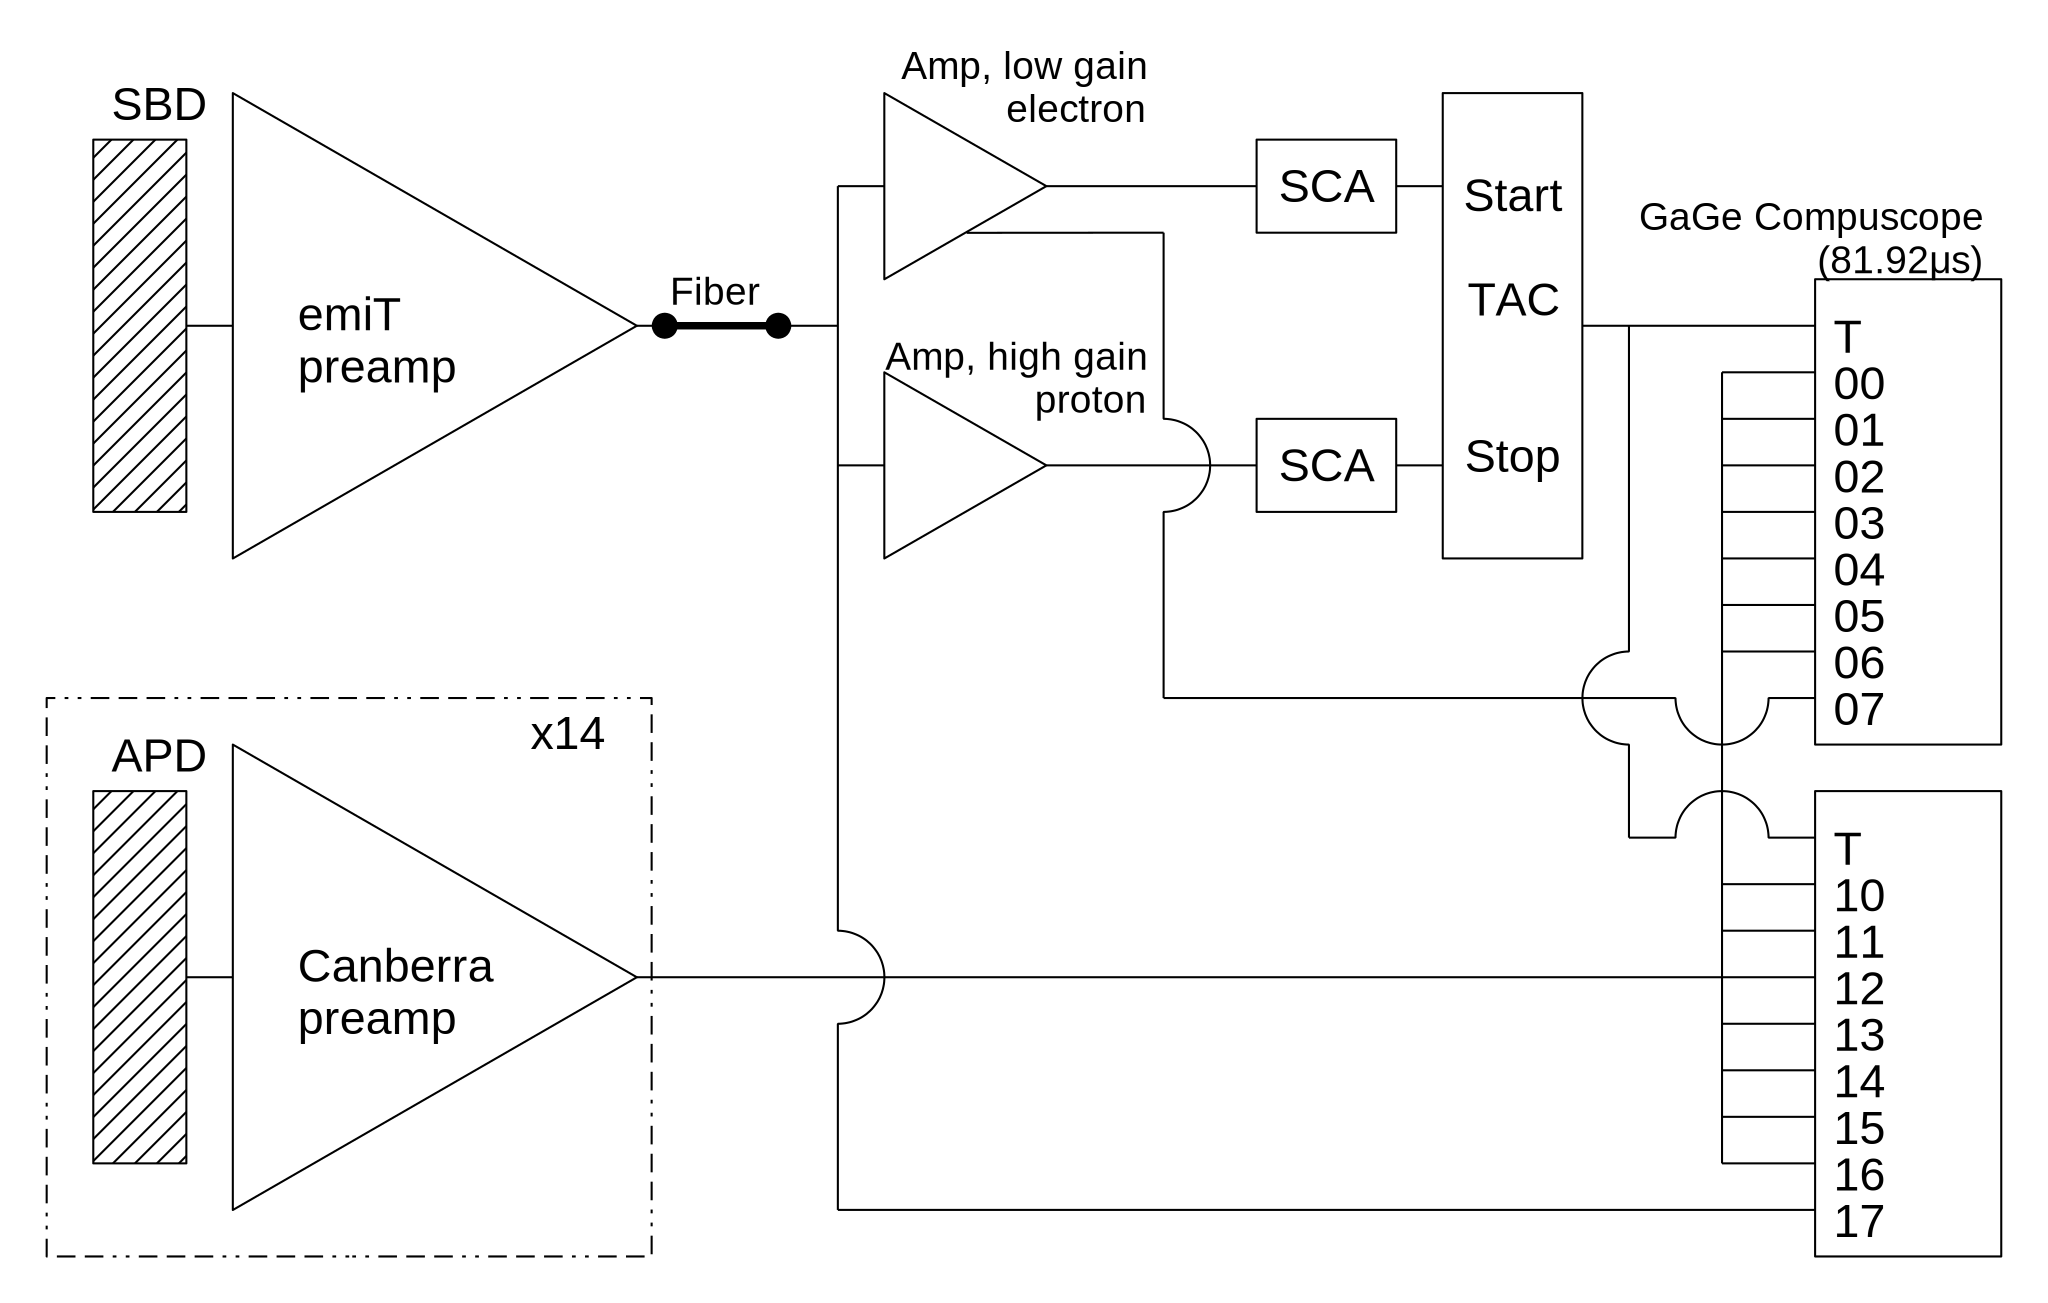
\includegraphics[width=\textwidth]{Electronics_schematic.png}
	\caption[Schematic of data acquisition system.]{Schematic of the data acquisition system used in the experiment. The charge particle SBD signal is split and amplified to yield start (electron) and stop (delayed) signals that are sent to a TAC. The TAC output triggers the GaGe oscilloscope card to allow the recording of both the SBD signal and the pre-amplified APD photon signal.}
	\label{fig:daq}
\end{figure}
The collected signal traces were buffered by the GaGe cards until full at which point the buffer would be flushed to the disc. Buffer sizes of 20 and 100 events were used at various times. For calibration runs, the cards would flush their buffers as soon as they were full. For standard runs, the buffers would only be flushed when both were full. The data were recorded in a file for each GaGe card, using just over 32~KB of storage per event per card in the following format:\par
\begin{itemize}
	\item A 5000 character header containing setting information;
	\item An entry for each event containing;
	\begin{itemize}
		\item An eight character delimiter;
		\item A 32-bit integer recording the number of the event within the buffer;
		\item A 64-bit floating-point timestamp;
		\item A 32-bit integer noting the number of channels (8);
		\item A 32-bit integer set to 255;
		\item Eight sets of 2048 16-bit integer signal traces;
	\end{itemize}
	\item A footer containing event counts and additional settings.
\end{itemize}\par
It was discovered after the completion of data collection that the digitizer cards had not been properly synchronized. This means that, while running in standard mode with the external trigger, the buffers will occasionally go out of sync and wait for the other card to fill before flushing to disc. Fortunately, the timestamps allowed this problem to be corrected, as discussed in Sec.~\ref{sec:timestamp}. For most runs, the triggered events that could not be corrected resulted in a dead time of less than 0.2\%. For a single series of runs (S305), a high trigger rate and a reduced digitizer buffer size resulted in a 5\% dead time.\par
This experiment was on the beam line at NIST from July of 2008 through November of 2009. During this time, the experiment ran for a total of 164.4 days. Approximately $9.7~\times ~10^7$ electron-proton events were recorded at all mirror voltages. A total of 25~TB of data was collected, including calibrations. The speed at which these data can be analyzed has largely been limited by the read capacity of the 1~TB hard drives used for storage. These drives have an average transfer rate of 25~MB/s or approximately 400 events per second. However, a new analysis workstation at Arizona State University has allowed us to greatly increase the analysis speed. This machine is equipped with five 3~TB hard drives in a software RAID 5 configuration and sixteen CPU cores. Although limitations in the ROOT libraries have prevented us from fully utilizing this computer, we can analyze all of the full mirror data (8.9~TB) in less than one day.

\chapter{DATA ANALYSIS}
\label{ch:analysis}
Unlike most experiments that simply record hardware triggers, RDK I and RDK II recorded digitized oscilloscope traces. An example of these traces is shown in figures~\ref{fig:bgo_signal_ch4} and~\ref{fig:bapd_signal_ch4} for the BGO and bAPD signals, respectively. This resulted in a large amount of data that had to be analyzed to extract meaningful parameters. To this end, two algorithms are being independently developed to extract meaningful parameters from the recorded waveforms. Jeff Nico, one of the leaders of the RDK I and II experiments at NIST, is developing one of these methods. The details of the other algorithm, developed by myself, is discussed in this chapter. Section~\ref{sec:photoanalysis} explains how a peak height and start time are determined for each photon detected. Section~\ref{sec:epanalysis} discusses how the same parameters are derived for the electron and proton signals. Section~\ref{sec:post_process} discusses further cuts and corrections to the data and Sec.~\ref{sec:background} describes how the uncorrelated background is removed from the data.\par
A comparison of the results of the two analyses with the Monte Carlo simulation can be found in Sec.~\ref{sec:results}.

\section{Photon signal analysis}
\label{sec:photoanalysis}
\begin{figure}[t]
	\includegraphics[width=\textwidth]{BGO_waveform.png}
	\caption[A typical BGO-APD signal with SBD signal.]{A typical BGO-APD signal with SBD signal. The blue line shows the slower pre-amplified output of the BGO coupled to the APD for a photon event occurring in coincidence with the electron. Events attributable to radiative decay photons occur as coincident events in the spectrum.}
	\label{fig:bgo_signal_ch4}
\end{figure}
An example of a BGO-APD (blue) and SBD (black) signal trace can be seen in Fig.~\ref{fig:bgo_signal_ch4}. This section details how the BGO-APD signals are analyzed to determine meaningful parameters from these traces. Note that while the examples of photon signals in this chapter show coincident events with the electron pulse, this is often not the case. While the electron and proton signals do not move much, the photon signals can be completely uncorrelated and shifted in either direction on the time axis.\par
A large amount of data was collected throughout the run of this experiment. To speed up analysis, only photon signals that are likely to be real events are fully analyzed. The criteria for likely events are as follows:\par
\begin{enumerate}
	\item the maximum of the signal trace (peak) is at least 300 digitizer units greater than the minimum of the signal trace;
	\item the peak follows the minimum;
	\item the peak is at least 5.12~$\mu$s (128 samples) before the end of the signal trace;
	\item the peak occurs long enough after the beginning of the signal to measure the baseline (192 samples or 7.68~$\mu$s for BGO-APD, 160 samples or 6.4~$\mu$s for bAPD);
	\item the maximum and minimum channels are within 300 units of the mean of the adjacent points;
	\item the peak is less than 30000 units.
\end{enumerate}\par
The uncertainty from digitizer noise on the measurement of any given sample is approximately 70 to 80 units. Thus, criteria 1 eliminates most null signals. Criteria 2 eliminates signals for which only the trailing edge of a photon event is recorded. Criteria 3 ensures that events that arrive too late for the peak to be observed are not analyzed. Criteria 4 ensures that there are enough points before the peak to enable a good fit on the signal before the photon event. Criteria 5 eliminates a class of pathological events where the spikes in voltage suggest hardware malfunctions. Criteria 6 eliminates events that exceed the voltage range of the digitizer.\par
\begin{figure}[t]
	\includegraphics[width=\textwidth]{bAPD_waveform.png}
	\caption[A typical bAPD signal with SBD signal.]{A typical bAPD signal with SBD signal. The blue line shows the fast rising pre-amplified output of the bAPD for a photon event occurring in coincidence with the electron. Events attributable to radiative decay photons occur as prompt events in the spectrum.}
	\label{fig:bapd_signal_ch4}
\end{figure}

\subsection{Baseline measurement}
\label{sec:baseline}
Because the signal can drift over time, a fast linear regression is used to determine the signal baseline. Because the starting time of the signal is not known, several regressions are needed over varying intervals. However, the constant interval between points allows the math of a linear regression to be simplified into a quick and efficient algorithm. In the two variable case ($y=\hat{\beta}_0+\hat{\beta}_1 x$), you can calculate $N-1$ regressions in $\mathcal{O}(N)$ operations. This will also provide useful information for determining the timing of the signal in a later section.\par
Starting from a linear regression with a polynomial fit function results in Eq.~\ref{eq:linreg1},
\begin{subequations}
	\label{eq:linreg1}
	\begin{align}
		\label{eq:linreg1a}
		Y &= X \hat{\beta}\\
		\label{eq:linreg1b}
		\hat\beta &= \left(X^T X\right)^{-1}X^T Y\\
		\label{eq:linreg1c}
		X_{ij} &= x_i^j,
	\end{align}
\end{subequations}
where $Y$ is a vector of the dependent variable (signal height at time $x_i$), $X$ is a matrix of the independent variable ($x_i^j$), and $\hat{\beta}$ is vector of the fit parameters. In the case were $x_i=i$, the product $(X^T X)$ is
\begin{equation}
	\label{eq:linreg2}
	\left(X^T X\right)_{ij}=\sum_k {\left(X^T\right)_{ik}X_{kj}}=
		\sum_k {X_{ki}X_{kj}}=\sum_k {x_k^{i+j}}=\sum_k {k^{i+j}}.
\end{equation}
In the two variable case, this becomes
\begin{equation}
	\label{eq:linreg3}
	X^T X=\sum_{k=0}^n {
		\begin{bmatrix}
			1 & k \\
			k & k^2
		\end{bmatrix}
	}=\begin{bmatrix}
		n+1 & \frac{n\left(n+1\right)}{2} \\
		\frac{n\left(n+1\right)}{2} & \frac{n\left(n+1\right)\left(2n+1\right)}{6}
	\end{bmatrix}.
\end{equation}
Thus, the inverse of Eq.~\ref{eq:linreg3} is
\begin{equation}
	\label{eq:linreg4}
	\left(X^T X\right)^{-1}=\frac{1}{n\left(n+1\right)\left(n+2\right)}
	\begin{bmatrix}
		2n\left(2n+1\right) & -6n \\
		-6n & 12
	\end{bmatrix}.
\end{equation}
Which yields the fitting matrix to be applied to the signal $Y$,
\begin{equation}
	\label{eq:linreg5}
	\left[\left(X^T X\right)^{-1} X^T\right]_{ij}
	=\sum_{k=0}^1\left[\left(X^T X\right)^{-1}\right]_{ik}j^k=
	\begin{bmatrix}
		\frac{2n\left(2n+1\right)-6nj}
			{n\left(n+1\right)\left(n+2\right)} \\
		\frac{-6n+12j}{n\left(n+1\right)\left(n+2\right)}
	\end{bmatrix}_i.
\end{equation}
Finally, the fit parameters $\hat\beta$ can be solved for as shown in Eq.~\ref{eq:linreg6}.\par
\begin{subequations}
	\label{eq:linreg6}
	\begin{align}
		\label{eq:linreg6a}
		\hat\beta_0&=\frac{2\left(2n+1\right)}
			{\left(n+1\right)\left(n+2\right)}\sum_{i=0}^n {Y_i}
			-\frac{6}{\left(n+1\right)\left(n+2\right)}\sum_{i=0}^n{iY_i}\\
		\label{eq:linreg6b}
		\hat\beta_1&=\frac{12}{n\left(n+1\right)\left(n+2\right)}\sum_{i=0}^n {iY_i}
			-\frac{6}{\left(n+1\right)\left(n+2\right)}\sum_{i=0}^n {Y_i}
	\end{align}
\end{subequations}
Because almost all of the calculations necessary to obtain the parameters of the $m$th regressions are necessary for the $n$th regression where $m~<~n$, these results can be obtained for very little CPU time. These additional fits will be useful later when determining the start time of the photon signal.\par
\subsection{Smoothing}
\label{sec:smooth}
\begin{figure}[t]
	\centering
	\includegraphics[width=0.8\textwidth]
		{Localregressionsmoother.png}
	\caption[Example of local regression smoothing]{Example of local regression smoothing. In this case, points were randomly generated around a sinusoidal signal and smoothed using a local linear regression. The original function is shown in green, the randomized points are blue, and the smoothed curve is red. The yellow area represents the weighting function used on the red points and the black line is the resulting fit~\cite{wiki:kernelsmooth}.}
	\label{fig:loess1}
\end{figure}
The signals are then smoothed by using a weighted sum derived from a local polynomial regression, a method commonly referred to as locally weighted scatterplot smoothing or LOWESS. An example of smoothing with a LOWESS method is shown in Fig.~\ref{fig:loess1}. Like the regression described above, the math can be simplified because of the regular interval between points. Thus, a weighting vector $\hat W\left(x_0\right)$ need only be calculated once for each time $x_0$,\par
%Need more text here.
\begin{subequations}
	\label{eq:loess1}
	\begin{align}
		\hat Y\left(x_0\right)&=\hat W\left(x_0\right) y\\
		\hat W\left(x_0\right)&=\hat{x_0}
			\left(X^T W\left(x_0\right)X\right)^{-1} X^T
			W\left(x_0\right)\\
		W_{ij}\left(x_0\right)&=\left(1-\left|
			\frac{x_i-x_0}{r+1}\right|^{p}\right)\delta_{ij}\\
		y^T&=\left(x_{-r},x_{-r+1},\ldots,x_{r}\right)\\
		\left(\hat{x_0}\right)_j&=x_0^j=\delta_{0j}\\
		X_{ij}&=x_i^j=i^j\quad\quad j\in\left[0,o\right],
	\end{align}
\end{subequations}
where $r$ is the smoothing radius, $p$ is the power of the weighting function, and $o$ is the order of the polynomial fit. In fact, $\hat W\left(x_0\right)$ need only be calculated $2r+1$ times because it is translationally invariant except at the ends of the signal.\par
Two smoothed signals are used in the signal analysis. For measuring the peak height, reducing random noise is more important than the structure of the signal, so a higher smoothing radius is used. In this case, a smoothing radius of 32, weight function power of 2, and a polynomial of order 1 (i.e. linear) were used. For determining the timing of the signal, a smaller smoothing radius must be used. In this case, a smoothing radius of 4, weight function power of 1, and a linear fit function were used. The parameters were chosen largely through trial and error in order to find a smoothing algorithm that would either preserve timing resolution or minimize signal noise. For later reference, these smoothed signals will be the E-smoothed and t-smoothed signals, respectively.\par
\subsection{Signal parameterization}
\label{sec:parameters}
Once the smoothed signals and baseline fit are generated, the timing and peak height parameters can be obtained. First, the peak channel and height of the E-smoothed signal is determined. Let us refer to these as $x_{max}$ and $E_{max}$, respectively. To first approximation, $E_{max}$ is the peak height of the signal. To further refine the measurement, the baseline and timing must be determined.\par
The signal is then traced back from $t~=~x_{max}$ until the sum of the squared residuals per degree of freedom of the baseline fit is less than 7000, approximately 10\% above the squared standard deviation that one would expect from the digitizer for a constant (flat) signal. Next, the program continues to trace back the signal until it falls below 10\% of the baseline-corrected peak height. This baseline is determined from the parameters from the fast linear regression discussed in Sec.~\ref{sec:baseline}. To minimize the contribution of the photo signal to the baseline fit, the baseline is measured at an offset. This offset is chosen based on the rise time of a typical signal. For a fast rising bAPD, an offset of 1.28~$\mu$s was used. For a slow rising BGO-APD, an offset of 2.56~$\mu$s was used.\par

\section{Charged particle signal analysis}
\label{sec:epanalysis}
The electron and proton parameters are calculated from the amplified SBD signal. First, the peak channel is determined along with the peak height. Because the amplified signal does not have the same voltage drift as the pre-amplified signals, the mean of the range outside of the electron and proton pulses is used as the baseline. The range used to calculate the baseline is from $0~\mu s~\leq~t~<t_e-5.12~\mu s$ and from $t_e+35.84~\mu s~\leq~t~<81.92~\mu s$ where $t_e$ is the electron peak time. The electron peak height is adjusted based on this baseline.\par
Next, the algorithm ignores the next 1.2~$\mu$s after the electron peak height and scans the signal until it is no longer descending. The signal is no longer descending when the signal at the current time is less than at each of the next four times. The signal is searched from this point until the end of the on peak window for a proton peak height and channel. This peak height is then adjusted by the baseline.\par
\section{Post-processing}
\label{sec:post_process}
In this section, further refinements to the data are considered. Section~\ref{sec:timestamp} explains how a synchronization issue between the two oscilloscope cards was corrected. Because multiple BGO detectors can trigger off of a single radiative decay, it was decided to sum the energies of these events into a single event as described in Sec.~\ref{sec:multiplicity}. Finally, additional cuts on the times and energies of these events are discussed in Sec.~\ref{sec:cuts}.
\subsection{Timestamp correction}
\label{sec:timestamp}
As mentioned in Sec.~\ref{sec:daq}, the GaGe oscilloscope cards were not properly synchronized during data collection. Fortunately, the timestamp information could be used to resynchronize the data in post processing. However, several issues complicated this effort.\par
First, one of the GaGe cards was found to have a single defective bit always set to one when recording the timestamp. Because the effect of this single bit (2\textsuperscript{32} samples or 170~s) was much larger than the average time between events (0.1~s), a bitwise mask filter to turn this bit off was applied to the first two timestamps on that card. Then, the masked timestamp for event $n$ was compared to the corrected timestamp for event $n-2$ and a threshold set to 2\textsuperscript{29} samples. If the masked timestamp fell within this range, the timestamp for that event was set to the masked value. This process is then repeated except each event $n$ is compared to the previous event $n-1$. This single bit correction was done in two phases because of the next timestamp issue: random timestamp ``glitches.''\par
It was discovered that sometimes an event would have a seemingly random timestamp. In this and the next phase of the timestamp corrections, a buffer of 100 events (the GaGe card buffer size for most runs) for each GaGe card was used. For each buffer, the timestamps of the first two events in this buffer were compared and the first event was moved to a ``glitch'' buffer if its timestamp was after the second one. This process was repeated until the first two events in the buffer were sequential. Then, as long as there were more than two events in the buffer, the timestamps of each of those events were compared. If the first timestamp was less than the second timestamp, the first event was moved to a temporary buffer. Otherwise the second event was put into the ``glitch'' buffer. Finally, when the buffer size was two, the first event was moved to the temporary buffer. If the second timestamp was less than or equal to the first timestamp, then the second event was also moved to the temporary buffer. Otherwise it was put into the ``glitch'' buffer. The temporary buffer was then transfered to the original buffer.\par
Finally, the events in each buffer are compared to each other to synchronize the events. For each event, the ratio of the differences in timestamps between events was compared to a threshold
\begin{equation}
\label{eq:timestamp}
\left|\frac{t_0-t^*_0}{t_1-t^*_1}-1\right|<threshold
\end{equation}
where $t_n$ is the timestamp of the current event on card $n$ and $t^*_n$ is the timestamp of the last synchronized event. For most events, the threshold was set to 10\textsuperscript{-4}, but this condition was relaxed a little to 10\textsuperscript{-3} for the first event as one card was often slower to start collecting data. If Eq.~\ref{eq:timestamp} was not satisfied, an empty event is inserted into the buffer in which $t_n-t^*_n$ is greater.\par
When all events in the run have been synchronized, the ``glitch'' buffers were added at to the end of the list of events. The ``glitches'' on each card are paired with an empty event.\par
Only events where both cards triggered properly and could be resynchronized were used in the analysis. For most runs, this results in a loss of approximately 0.2\% of events. For a single series of runs (S305), a smaller GaGe card buffer size and an unusually high trigger rate resulted in 5\% of events being lost to improper synchronization.
\subsection{Multiplicity}
\label{sec:multiplicity}
Because there are multiple detectors, it would be useful to sum the energy deposited for coincident photon events. To this end, after the cards have been resynchronized, photon events are collected into nearly coincident groups of multiplicity $M$ where $M$ is the number of photons in that group. For each event where one or more photons above 10~keV are detected in the BGO detectors, those photons are put into a list and sorted by their times $t_\gamma$. These photons are then tagged such that if the difference in $t_\gamma$ between two sequential photons is less than 600~ns then those photons are within the same group. The number of photons in each group are then counted and have their multiplicity set to that number.\par
When the events are binned into histograms later on, the photon energy is summed up over all events in the same group. Also, the time is averaged over that group. Finally, each event is weighted by $1/M$ in each photon detector that registered. Thus, when the detectors are summed, each group counts as a single photon event.

\subsection{Additional cuts}
\label{sec:cuts}
\begin{figure}
	\centering
	\includegraphics[width=\textwidth]{TraceBad.png}
	\caption[False trigger event.]{A false trigger event. High energy gamma rays can strike the SBD causing a signal with a long trailing edge (see above). This signal satisfies the hardware trigger but is not an electron-proton event.}
	\label{fig:cooper1}
\end{figure}
After the electron, proton, and photon parameters were calculated, the data were further filtered to remove false coincidence events. The following cuts are made when determining valid electron-proton triggers:
\begin{itemize}
	\item $2~\mu s~<~t_p-t_e~<~25~\mu s$;
	\item $50~keV~<~E_e~<~800~keV$;
	\item $7~keV~<~E_p~<~31~keV$.
\end{itemize}
The upper limit on the electron-proton time of flight (TOF) determined by the hardware cutoff for the trigger (see Sec.~\ref{sec:daq}) while the lower bound ensures that the proton signal does not ride on the electron pulse. The lower electron energy is set to be above the hardware trigger threshold to minimize the effect of gain drift on the SBD. The upper limit of the proton energy was chosen to be below the limits imposed by the hardware to exclude double electron events.\par
The following cuts are placed on the photon detection data:
\begin{itemize}
	\item BGO : $10~keV~<~E_\gamma~<~800~keV$,
	\item bAPD : $250~eV~<~E_\gamma~<~20~keV$.
\end{itemize}\par
The lower energy limits on both the BGO and bAPD energy were chosen to be as low as possible while ensuring that the signal analysis algorithm can still distinguish real events from noise.\par
It is possible for high energy background particles to strike the SBD and produce a signal with a long trailing edge (see Fig.~\ref{fig:cooper1}). These signals satisfy the hardware trigger, but are likely to be beam related gamma rays. Discussion continues on how best to identify these events. For the moment, this analysis does not attempt to cut these events.\par
%electron and proton cuts
%cooper cut
%tbd

\section{Background Subtraction}
\label{sec:background}
\begin{figure}[t]
	\centering
	\subfloat[On-peak spectrum]{
		\includegraphics[width=0.48\textwidth]
			{on_peak_bgo_sum.png}
		\label{fig:onpeak_bgo}
	}
	\subfloat[Off-peak spectrum]{
		\includegraphics[width=0.48\textwidth]
			{off_peak_bgo_sum.png}
		\label{fig:offpeak_bgo}
	}\par
	\subfloat[Background subtracted spectrum]{
		\includegraphics[width=0.48\textwidth]
			{bgc_bgo_sum.png}
		\label{fig:bgc_bgo}
	}
	\subfloat[Timing windows]{
		\includegraphics[width=0.48\textwidth]
			{delta_t_bgo_sum.png}
		\label{fig:delta_t_bgo}
	}
	\caption[BGO observed energy and timing spectra.]
		{The observed energy and timing spectra for the BGO data. (a) The on-peak energy spectrum. (b) The off-peak energy spectrum. (c) The background subtracted energy spectrum (on-peak minus scaled off-peak). (d) The timing windows, where on-peak is between the red lines and off-peak is outside the red lines. The vertical axis is the ratio of electron-proton-photon events to electron-proton triggers. The horizontal axis in (a) through (c) is the photon energy in keV from 0~keV to 800~keV. The horizontal axis in (d) is the difference in photon and electron time in $\mu$s from -10~$\mu$s to 22~$\mu$s.}
	\label{fig:bgo_results}
\end{figure}
\begin{figure}[t]
	\centering
	\subfloat[On-peak spectrum]{
		\includegraphics[width=0.48\textwidth]
			{on_peak_bapd_sum.png}
		\label{fig:onpeak_bapd}
	}
	\subfloat[Off-peak spectrum]{
		\includegraphics[width=0.48\textwidth]
			{off_peak_bapd_sum.png}
		\label{fig:offpeak_bapd}
	}\par
	\subfloat[Background subtracted spectrum]{
		\includegraphics[width=0.48\textwidth]
			{bgc_bapd_sum.png}
		\label{fig:bgc_bapd}
	}
	\subfloat[Timing windows]{
		\includegraphics[width=0.48\textwidth]
			{delta_t_bapd_sum.png}
		\label{fig:delta_t_bapd}
	}
	\caption[bAPD observed energy and timing spectra.]
		{The observed energy and timing spectra for the bAPD data. (a) The on-peak energy spectrum. (b) The off-peak energy spectrum. (c) The background subtracted energy spectrum (on-peak minus scaled off-peak). (d) The timing windows, where on-peak is between the red lines and off-peak is outside the red lines. The vertical axis is the ratio of electron-proton-photon events to electron-proton triggers. The horizontal axis in (a) through (c) is the photon energy in keV from 0~keV to 20~keV. The horizontal axis in (d) is the difference in photon and electron time in $\mu$s from -13.84~$\mu$s to 11.76~$\mu$s.}
	\label{fig:bapd_results}
\end{figure}
If the difference between the photon and electron times is plotted (Fig.~\ref{fig:delta_t_bgo} and Fig~\ref{fig:delta_t_bapd}), you can readily see a correlation between electron and photon. Ideally, these events should be coincident, but delays in the electronics cause the electron signal to be delayed about 1~$\mu$s. In addition, noise on the signal broadens the coincidence peak. Finally, because the timing is determined at the point where the signal reaches one tenth its peak height, higher energy photons are often recorded late due to the slope of the signal. Thus the coincidence peak has a trailing edge. In practice, an ``on-peak'' window is defined around the coincidence peak. These events are labeled as radiative decay events.\par
As shown in Fig.~\ref{fig:delta_t_bgo} and Fig.~\ref{fig:delta_t_bapd}, there is a uniform spectrum of uncorrelated events. Because this background is uniform, the average of ``off-peak'' windows can be scaled and subtract out of the ``on-peak'' window. Thus, the background corrected number of electron-delayed proton-photon coincidence events ($R_{eqg}$) is\par
\begin{equation}
	\label{eq:bg_sub}
	R_{epg}=\sum_\textrm{on-peak}N_{ep\gamma}
		\left(\Delta t\right)-\frac{\Delta t_\textrm{on-peak}}
		{\Delta t_\textrm{off-peak}}\sum_\textrm{off-peak}N_{ep\gamma}
		\left(\Delta t\right),
\end{equation}
where $N_{ep\gamma}\left(\Delta t\right)$ is the number of electron-delayed proton events with a photon event $\Delta t$ after the electron and $\Delta t_\textrm{on~peak}$ and $\Delta t_\textrm{off~peak}$ are the widths of the on-peak and off-peak windows, respectively. Similarly, this can be applied to each energy bin to obtain the background subtracted energy spectrum.
%On peak, off peak, background subtracted figures
\chapter{CALIBRATIONS AND SYSTEMATICS}
\label{ch:calibration}
The ambitious goals of the RDK II experiment, obtaining the radiative decay branching ratio with a 1\% overall precision and the photon energy spectrum within a few percent, require an understanding of systematic uncertainties better than an order of magnitude beyond the level achieved in the RDK I measurement. In this chapter the contributions to the systematic uncertainties from the detector elements and the electrostatic mirror are addressed. The detectors main contributions to systematic uncertainties come from gain shifts during the year long measurement, temperature effects, and effects of magnetic fields on the APDs. Sections~\ref{sec:bgo_cal} and~\ref{sec:bapd_cal} present the work carried out to perform the photon energy calibrations from the BGO array and the bare APDs, respectively. Section~\ref{sec:sbd_cal} discusses the calibration of the electron and proton signals as obtained from the surface barrier detector (SBD). Section~\ref{sec:mirror_syst} discusses the issues connected with the operation of the electrostatic mirror.

\section{BGO-APD Calibrations}
\label{sec:bgo_cal}
\begin{figure}[t]
	\includegraphics[width=\textwidth]{c256offPeak.png}
	\caption[Observed spectra from a set of \emph{in situ} calibration runs.]{Observed spectra from a set of \emph{in situ} calibration runs. Top row from left to right: detectors 00 through 03. Second row: detectors 04 through 06. Third row: detectors 10 through 13. Forth row: detectors 14 through 16. Detectors 02, 06, and 16 were bAPD detectors. The rest were BGO-APD detectors.}
	\label{fig:calspec}
\end{figure}
Calibrations of the BGO-APD detectors were done both while on the beam line and after removal of the experiment from the guide hall. At the beginning of each run and every twelve hours thereafter, the data acquisition system (DAQ) was put into calibration mode for 30 minutes. While in calibration mode, instead of triggering only on the electron-delayed proton events the DAQ triggers on all detectors. This mode provides a spectrum of photons in which the 511~keV photons from electron-positron annihilation forms an easily identifiable peak as seen in Fig.~\ref{fig:calspec}. This peak can be fitted to a Gaussian function on an exponentially decaying background with low (0.4\%) statistical uncertainty. The origin and this point, calculated for each calibration run, were used to convert from units of voltage to energy.\par
After data collection was complete, the experiment was moved to another building at NIST for off beam calibrations and storage. For these runs, a steel tube (with an inner radius of 1.23~cm and an outer radius of 1.27~cm) wrapped in insulating aluminized mylar was placed along the center of the detector. By using this setup, data were collected from radioactive sources placed within the detector. Figure~\ref{fig:cs137_v_mc} shows some of the data collected with a \textsuperscript{137}Cs source. More calibrations were conducted with \textsuperscript{57}Co, \textsuperscript{133}Ba, and \textsuperscript{241}Am sources. These runs were used to refine the energy deposition functions used in the Monte Carlo simulations.\par
\begin{figure}[t]
	\includegraphics[width=\textwidth]{cs137_v_mc.png}
	\caption[Comparison of Cs-137 calibration data with Monte Carlo.]{A comparison of the \textsuperscript{137}Cs with the Monte Carlo simulation. The background spectrum was measured during a run with no sources. The prediction includes the Monte Carlo results plus the background.}
	\label{fig:cs137_v_mc}
\end{figure}

\subsection{Temperature dependence}
\label{sec:bgo_temp}
\begin{figure}[p]
	\centering
	\includegraphics[width=0.89\textwidth]
		{Layout_gain_temp_comp_424.jpg}
	\caption[Results of warm up/cool down calibration run.]
		{The results of the warm up and cool down calibration run. The upper left figure shows the temperature over time. The detectors are situated between the upstream (blue) and downstream (green) temperature senors. The lower left figure shows position of the calibration peak, nominally 662~keV, for various detectors. The spikes from about run 300 to run 600 are the results of the automated fit function failing to find the calibration peak. The right hand figures show the temperature corrected (colored) and uncorrected (black) peak positions. The upper right figure is a magnification of the lower right.}
	\label{fig:tempgain}
\end{figure}
It has been known for some time that the gain and breakdown voltage of APDs are dependent on their operating temperature~\cite{moszynski03}. To counteract this effect, the APD voltages were adjusted periodically to ensure that the 511~keV calibration peak was in the same position. In addition, temperature sensors were placed on the LN\textsubscript{2} and LHe reservoirs and the upstream and downstream ends of the detector. When the experiment was taken off beam, the detector was allowed to warm up and then cool down while running with the \textsuperscript{137}Cs source (see Fig.~\ref{fig:tempgain}). From these data, it was found that the APD gain decreased between 5~\%/K and 8~\%/K and the breakdown voltage increased between 1~V/K and 1.5~V/K ~\cite{Cooper201264}. These changes originate mainly from the temperature dependence of the APD, as BGO light output decreases <~1~\%/K near 100~K ~\cite{gironnet08}. With this knowledge, it is possible to extrapolate between calibration runs to find a calibration peak for each run of the experiment.

\subsection{Positional dependent gain}
\label{sec:bgo_position}
\begin{figure}[t]
	\centering
	\includegraphics[width=0.95\textwidth]{position_dep.png}
	\caption[Positional dependent light output of BGO scintillators.]{The positionally dependent light output of BGO scintillators created by stepping several radioactive sources through the detector. Vertical axis shows the peak height of the calibration source relative to the peak height at the center of the detector (at approximately 23~cm). These measurements were done for collimated (solid line) and uncollimated (dashed line) sources.}
	\label{fig:posgain}
\end{figure}
As demonstrated in Ref.~\cite{keil70}, the geometry of a scintillator and photon detector can influence the light output. Two collimators were constructed to measure the positional dependence of the light yield of the BGO crystals. One was made of 1~mm Cd foil with a 1.6~mm ring opening and another with two layers of 2.5~mm Pb foil with a 2~mm ring opening. Both the collimated and uncollimated \textsuperscript{241}Am, \textsuperscript{57}Co, and \textsuperscript{133}Ba sources were stepped through the detector in 5~mm increments. An uncollimated \textsuperscript{137}Cs source was also used, but no collimator that could block all of the 662~keV gamma rays could fit within the reentrant tube. The results of these tests can be seen in Fig.~\ref{fig:posgain}. The relative gain was defined to be 1 near the center of the BGO. These measurements are consistent with the calculations done in Ref.~\cite{keil70}. A fit of the positional dependence of the light yield was incorporated into the energy deposition functions within the simulations.

\section{bAPD Calibrations}
Similarly to the BGO-APD detectors, the bAPD detectors were calibrated by using a fit based on the peak from a source of known energy. In this case, an attenuated \textsuperscript{55}Fe source was placed near the detector. The 5.9~keV X-rays from this source were used as the calibration point for these detectors in much the same way as the 511~keV electron-positron annihilation peak was used to calibrate the BGO-APD detectors.\par
Unlike the BGO-APD detectors, the bAPD detectors were not tested in the off-beam setup as the steel tube plus shielding blocked most X-rays below 30~keV. Instead, one of these detectors was placed in a test Dewar as described in Ref.~\cite{gentile12a}. This apparatus was placed on the Synchrotron Ultraviolet Radiation Facility (SURF) at NIST in an attempt to model the APD response to low energy X-rays. The response of the APD to the SURF spectrum was too complex to develop a satisfactory model. The next step was to take the apparatus and one APD to the U3C monochromatic beam line at Brookhaven National Laboratory (BNL). From these data, a model of the detector's collection efficiency as a function of penetration depth was developed (see Fig.~\ref{fig:colleff}). This model proved to be robust enough to predict the results of the SURF testing for another APD from the same batch, requiring only minimal adjustments to the parameters. However, the third APD was from a newer batch with a different doping profile and required a non-linear scaling term as described in Ref.~\cite{gentile12a}.\par
\label{sec:bapd_cal}
\begin{figure}[t]
	\centering
	\subfloat[Collection efficiency model for bAPD 1 as a function of penetration distance.]{
		\includegraphics[width=0.47\textwidth]{colleff1.pdf}
	}
	~
	\subfloat[Collection efficiency times gain for bAPD 3 as a function of penetration distance.]{
		\includegraphics[width=0.47\textwidth]{colleff2.png}
	}
	\caption[Direct detector collection efficiency.]{The model of the direct detector gain and collection efficiency (vertical axis) as a function of penetration depth (horizontal axis)~\cite{gentile12a}.}
	\label{fig:colleff}
\end{figure}

\subsection{Magnetic field effects}
\label{sec:bapd_field}
When this experiment was conceived, it was believed that APDs were insensitive to magnetic fields. However, when a four-APD configuration with the APDs facing the beam was tested, some anomalous features were observed in the spectra. Because these issues had not been observed in the BGO-APD detectors, it was decided to change the configuration such that the surface of the bare APDs would be parallel to that of the BGO-APDs. This arrangement eliminated the anomalies and allowed the experiment to proceed concurrently with a study of the effects of magnetic fields on APDs at cryogenic temperatures~\cite{gentile11}.\par
To test these effects, one of the large area APDs was placed in an apparatus in which the temperature and magnetic field could be varied from 77~K to 250~K and between 0~T to 4.6~T, respectively. It was found that the effect of increasing the magnetic field at a given temperature was similar to the effect of decreasing the temperature for a given magnetic field. The conclusion of this experiment was that X-rays absorbed in the drift region of the APD produce fewer photoelectrons than those absorbed in the depletion region when at cryogenic temperatures and with magnetic fields perpendicular to the electric fields.\par

\section{SBD Calibrations}
\label{sec:sbd_cal}
\begin{figure}[t]
	\includegraphics[width=\textwidth]{G_ePkHt_1.png}
	\caption[SBD peak height calibration fit.]{SBD peak height calibration fit and residuals. The electron spectrum (red) from each series was fitted to a model of the electron endpoint energy (black). The horizontal axis shows the peak height in the oscilloscope units. The residuals of this fit are shown in the upper section.}
	\label{fig:sbd_cal}
\end{figure}
The surface barrier detector (SBD) was calibrated by using a fit on the endpoint of the electron energy spectrum (see Fig.~\ref{fig:sbd_cal}). Electron and proton peak heights were then scaled such that the electron energy endpoint is at 756.58~keV (the physical endpoint, 781.58~keV, less 25~keV from the SBD potential).\par
Additionally, radioactive sources were used periodically throughout the data collection. Samples of either \textsuperscript{241}Am or \textsuperscript{57}Co were placed within the detector for some calibration runs. Combined with the origin and the endpoint, these four calibration points showed that the SBD electronics were non-linear. To account for this effect, data were collected with an electronic pulser attached to inputs of the SBD electronics at various points. The results of these linearity checks were included in the Monte Carlo simulation described in chapter~\ref{ch:mc}

\section{Electrostatic Mirror}
\label{sec:mirror_syst}
\begin{figure}[t]
	\includegraphics[width=\textwidth]{mirror_ep_e.png}
	\caption[Effect of electrostatic mirror voltage on the ep/e ratio.]{The effect of electrostatic mirror voltage on the ep/e ratio. The upper orange double line represents the simulation. The non-orange points represent the data collected in January and February of 2009 corrected for the non-decay (magnet off) electron rate. The lower orange double line with star points is the simulation shifted right by +65~V and down by -0.055.}
	\label{fig:mirror_ep_e}
\end{figure}
Throughout the running of the experiment, several series of data were collected with the electrostatic mirror below full voltage (1400~V). It was hoped that these data would be useful in benchmarking the simulations. However, it was found that the ratio of $R_{ep}/R_e$ was not consistent before and after a detector warm up for low voltages on the mirror. Further investigation showed that the ratio as a function of voltage looked as if the mirror voltage was incorrect. Figure~\ref{fig:mirror_ep_e} shows one such voltage scan. In this case the mirror appeared to be 65~V below the high voltage setting. Other scans showed similar features with varying voltage offsets. A wire to measure the mirror voltage was added and showed no deviations from the high voltage settings. It is believed that some ungrounded object near the mirror was becoming charged and acting as a second mirror. Fortunately, when operating at the full mirror potential, this effect becomes negligible as all protons heading downstream are reflected. The partial mirror data that was collected has been disregarded.

\chapter{SIMULATIONS}
\label{ch:mc}
Calculation of the effective solid angle of the RDK detector is complicated by the electron and proton interaction with the electromagnetic fields. Furthermore, secondary reactions such as Compton scattering and x-ray florescence distort the photon energy spectrum. This chapter focuses on the Monte Carlo simulation used to understand these interactions and extract a branching ratio. Section~\ref{sec:mcgen} presents the method used to generate realistic sample events. Section~\ref{sec:mctrack} describes how these events propagate through the simulated detector. Section~\ref{sec:mcfield} deals with the calculation of the electric and magnetic fields and its implementation into the Monte Carlo code. Section~\ref{sec:mcdetresp} describes how the generated events are observed by the detectors. Finally, Sec.~\ref{sec:mcresults} shows comparisons of the Monte Carlo simulation with data taken from the neutron beam and radioactive sources.

\section{Event Generator}
\label{sec:mcgen}
Approximately 300 million three-body (electron, proton, and anti-neutrino)~\cite{jackson57} and four-body (including photon) events were generated by using a von Neumann rejection method. In this method, a probability function $P_8$ is defined as the differential decay rate (Eq.~\ref{eq:vn1}). The maximum value of $P_8$ is designated as $M$.
\begin{equation}
	\label{eq:vn1}
	\frac{d^8\Gamma}{dE_e d\Omega_e d\omega d\Omega_{\gamma}
		d\Omega_{\bar{\nu}}}=P_8\left(E_e,\cos\theta_e,\phi_e,
		\omega,\cos\theta_\gamma,\phi_\gamma,\cos\theta_{\bar{\nu}}
		,\phi_{\bar{\nu}}\right).
\end{equation}
To uniformly sample the available phase space, events are generated such that they are uniformly distributed into a $4\pi$ solid angle for each of the electron, photon, and anti-neutrino. Specifically, values of $\phi$ and $\cos\theta$ are generated such that they are uniformly sampled in the range of $\left[-\pi,\pi\right]$ and $\left[-1,1\right]$, respectively. The energy of the electron (including the rest mass) is also sampled uniformly within the range $m_e$ to the endpoint energy $E_0$ where
\begin{equation}
	\label{eq:vn2}
	E_0=\frac{m_n^2-m_p^2+m_e^2}{2m_n}\approx 1.3 MeV.
\end{equation}
The photon energy $\omega$ is uniformly sampled within the range $\left[\omega_t,\omega_{max}\right]$ where $\omega_t$ is the detector threshold and $\omega_{max}$ is the upper limit. From these parameters and the kinematic constraints, the anti-neutrino energy can be calculated as
\begin{equation}
	\label{eq:vn3}
	E_{\bar{\nu}}=\frac{m_n^2-m_p^2+m_e^2
		-2m_n\left(E_e+\omega\right)-2\left|\mathbf{p}_e\right|
		\omega\cos\theta_{e\gamma}}{2\left(m_n-E_e+\omega
		+\left|\mathbf{p}_e\right|\cos\theta_{e\bar{\nu}}
		+\omega\cos\theta_{\bar{\nu}\gamma}\right)},
\end{equation}
where $\theta_{ij}$ is the angle between particle $i$ and $j$. The same method applies to non-radiative decays where $\omega = 0$. To ensure that $E_{\bar{\nu}}\geq 0$, the upper limit of the photon energy is set to $\omega_{max}$ given by
\begin{equation}
	\label{eq:vn4}
	\omega_{max}=\frac{m_n^2-m_p^2+m_e^2-2m_n E_e}
		{2m_n+2\left|\mathbf{p}_e\right|\cos\theta_{e\gamma}}.
\end{equation}
Conservation of energy and momentum can be used to calculate the proton energy and momentum.\par
With the phase space uniformly sampled as described above, the probability $P_8$ is calculated from Eq.~\ref{eq:vn1}. The ratio $P_8/M$ is then compared to a random number $r\in\left[0,1\right]$ and events are rejected where $P_8/M>r$.\par

\section{Tracking}
\label{sec:mctrack}
The path of particles through the detector can be determined by integrating the equation of motion. Photons are trivial to track as their trajectories are not influenced by electric and magnetic fields. However, the paths of electrons and protons are not easily solvable and must be approximated numerically.\par
Two such algorithms were used the simulations. Geant4~\cite{geant4-nima} was used in one simulation while a custom tracker (referred to as MRK) was used in the other. Both use fourth order Runge-Kutta to numerically integrate the differential equations~\cite{press07}. With this method, an arbitrary differential equation $\dot{y}=f\left(t,y\right)$ can be solved by taking small time steps $h$ as described in Eq.~\ref{eq:rungekutta}. From a given set of initial conditions, $y_0$ and $t_0$, the value of $y_n$ can be found by iteratively stepping in increments of $h$ along the time axis.\par
\begin{subequations}
\label{eq:rungekutta}
\begin{align}
	&\dot{y}=f\left(t,y\right),\;y\left(t_0\right)=y_0\\
	&y_{n+1}=y_n+\frac{1}{6}\left(k_1+2k_2+2k_3+k4\right)\\
	&t_{n+1}=t_n+h\\
	&k_1=hf\left(t_n,y_n\right)\\
	&k_2=hf\left(t_n+\frac{1}{2}h,y_n+\frac{1}{2}k_1\right)\\
	&k_3=hf\left(t_n+\frac{1}{2}h,y_n+\frac{1}{2}k_2\right)\\
	&k_4=hf\left(t_n+h,y_n+k_3\right)
\end{align}
\end{subequations}
The resulting error is on the order of $h^5$ per step for an accumulated error on the order of $h^4$.\par
Because the proton's kinetic energy is much less than its mass, the equation of motion is described by the non-relativistic Lorentz force law
\begin{subequations}
\label{eq:nrlorentz}
\begin{align}
	\frac{d\mathbf{v}}{dt} &=\frac{q}{m}\left[
		\mathbf{E}+\mathbf{v}\times\mathbf{B}\right]\\
	\frac{d\mathbf{r}}{dt} &=\mathbf{v},
\end{align}
\end{subequations}
where $m$ and $q$ are the mass and charge of the proton, and $\mathbf{E}$ and $\mathbf{B}$ are the electric and magnetic fields.\par
In the case of electrons the relativistic Lorentz force must be applied. In the lab frame, the equation of motion becomes,
\begin{subequations}
\begin{align}
	\label{eq:rellorentz}
	\frac{d\mathbf{v}}{dt}&=\frac{e}{\gamma m_e}\left[
		\mathbf{E}-\left(\mathbf{E}\cdot\frac{\mathbf{v}}{c}\right)
		\frac{\mathbf{v}}{c}+\mathbf{v}\times\mathbf{B}\right]\\
	\frac{d\mathbf{r}}{dt}&=\mathbf{v},
\end{align}
\end{subequations}
where $\gamma=1/\sqrt{1-v^2/c^2}$. The initial conditions for each particle is taken from the list of events generated as described in Sec.~\ref{sec:mcgen}.\par
Approximately 20\% of the events tracked through the detector result in an electron-delayed proton conincidence trigger.

\section{Field Calculations}
\label{sec:mcfield}
\begin{figure}[t]
	\includegraphics[width=\textwidth]{mesh.png}
	\caption[Surface mesh used in Opera-3d.]{A bottom up view of the surface mesh generated by Opera-3d for the detector geometry. The magnet is drawn in green, the bore is in light blue, and the SBD BeO tube in magenta. The blue represents the slice of the detector in which the fields (not shown) are to be plotted.}
	\label{fig:mesh}
\end{figure}
An accurate simulation of electron and proton trajectories requires a fine mesh field map of the electric and magnetic fields. The calculations currently used in the Monte Carlo are the same ones used in the RDK I experiment. The magnetic fields were calculated by using a commercial software package~\cite{biotsavart} that numerically integrates the Biot-Savart law over a set of specified coil and wire configurations. The lack of magnetic materials within the bore results in a very accurate calculation. The coil configurations are known very precisely (see Table~\ref{tab:magnet}). A program was written to calculate the electric fields from first principles as described in Ref.~\cite{thesis:cooper}.\par
A new calculation of the electric and magnetic fields is now in development. This calculation is being developed with the TOSCA Static Field Analysis Program within Opera-3d by Vector Fields Software~\cite{opera3d}. This program uses an advanced finite element numerical analysis procedure that allows users to create models with complicated conductor geometry and user defined material properties. TOSCA then calculates the electrostatic and magnetostatic fields from fixed potential boundaries and current sources, respectively.\par
The values used for the relative permittivity and conductivity of the materials with the experiment are given in Table~\ref{tab:materials}. Some of these values were set to zero in the calculation because of complications in the way TOSCA handles thin materials with low conductivity between two different potentials. This issue was resolved by setting the conductivity of materials with below 10\textsuperscript{-6}S/m to zero.\par
After creating the model from primitive shapes with union and intersection like boolean functions, the background is defined and the model is meshed (Fig.~\ref{fig:mesh}). Once the model is built and meshed, the TOSCA analysis begins. The algorithm is based on a scalar potential formulation. TOSCA calculates the electric ($\mathbf{E}$) and magnetic field intensity ($\mathbf{H}$) from the electric potential ($V$) and magnetic scalar potential ($\phi$), respectively, as follows,
\begin{subequations}
	\begin{equation}
		\mathbf{E}=-\nabla V
	\end{equation}
	\begin{equation}
		\mathbf{H}=-\mu\nabla\phi
	\end{equation}.
\end{subequations}
Applying Maxwell's equations to these fields yields a set of equations
\begin{subequations}
	\begin{equation}
		\nabla\cdot\mathbf{D}=\nabla\cdot\epsilon\mathbf{E}=\epsilon\nabla^2 V=-\rho
	\end{equation}
	\begin{equation}
		\nabla\cdot\mathbf{H}=\mu\nabla^2\phi=0.
	\end{equation}
\end{subequations}
These Poisson's equations can be solved by using finite element methods. In most simulations, the reduced potential formulation for magnetic fields introduces large errors which propagate into the computed fields. However, this particular issue arises solely from the inclusion of currents flowing in magnetic materials. Because there are no magnetic materials within the detector, this is not an issue within the context of the RDK II simulation.
\begin{table}[t]
	\centering
	\begin{tabular}{|l|l|l|} \hline
		Material & Relative & Conductivity\\
		& Permittivity & (S/cm) \\\hline
		304 Stainless Steel & $1.00\times 10^{-15}$ & $8620.138888$ \\\hline
		Aluminum & $1.00\times 10^{-15}$ & $3.5\times 10^{5}$ \\\hline
		BeO & $6.7$ & $1.00\times 10^{-15}$ * \\\hline
		BGO & $44$ & $1.00\times 10^{-7}$ * \\\hline
		Brass & $1.00\times 10^{-15}$ & $1.56\times 10^{5}$ \\\hline
		Copper & $1.00\times 10^{-15}$ & $5.96\times 10^5$ \\\hline
		G10 & $4.6$ & $2.3406\times 10^{-14}$ \\\hline
		Lead & $1.00\times 10^{-15}$ & $4.55\times 10^4$ \\\hline
		Silicon & $11.68$ & $1.56\times 10^{-5}$ * \\\hline
		Teflon & $2.1$ & $1.00\times 10^{-26}$ * \\\hline
	\end{tabular}
	\caption[Table of materials and electrostatic properties.]{Table of the materials and their electrostatic properties used in the new field calculations. Those values marked by an asterisk were set to zero due to limitations within TOSCA.}
	\label{tab:materials}
\end{table}

\section{Detector Response}
\label{sec:mcdetresp}
When a particle is found to have entered a material, the simulation models the interaction with that material. Several software packages were used to model those interactions. In the MCNP simulation, the photon energy deposition, electron energy deposition, and backscattering were modeled with the MCNP5 and Penelope~\cite{Prasad1976103} libraries. For proton energy deposition, SRIM-2011~\cite{Ziegler1988215} was used. In the Geant4 simulation, all materials were modeled with the Geant4 Livermore libraries. These libraries allow for the modeling of several interactions including Compton scattering, ionization, and x-ray florescence.\par
After the deposited energy is calculated, several corrections are applied to the final energy. In BGOs, a correction is applied based on the position of the incident photon to account for the effects observed in Sec.~\ref{sec:bgo_position}. Another correction is applied to account for the non-linearity of the detectors. The results of this fit can be seen in Fig.~\ref{fig:cs137_v_mc}.\par
For the bAPDs, a gain and efficiency model were used to determine the observed energy. A description of this correction can be found in Sec.~\ref{sec:bapd_cal} and Ref.~\cite{gentile12a}.

\section{Comparison with Data}
\label{sec:mcresults}
\begin{figure}[t]
	\includegraphics[width=\textwidth]{e_energy_comparison.png}
	\caption[Comparison of electron energy spectrum with Monte Carlo.]{A comparison of the electron energy spectrum with the Monte Carlo simulation. The data and simulation are normalized such that the integral of each histogram is equal to one. The data in this plot were histogrammed with a 5~keV bin size while the Monte Carlo is shown with 1~keV bins.}
	\label{fig:ee_vs_mc}
\end{figure}
\begin{figure}[t]
	\includegraphics[width=\textwidth]{ep_tof_comparison.png}
	\caption[Comparison of the electron-proton time of flight with the Monte Carlo.]{A comparison of the electron-proton time of flight with the Monte Carlo simulation. The data and Monte Carlo are normalized such that the integral of each graph is equal to one. Both graphs were made with a 40~ns bin size.}
	\label{fig:ep_tof_vs_mc}
\end{figure}
The results of the Monte Carlo simulation have repeatedly been benchmarked against the data to ensure an understanding of how the detector works. A comparison of the electron energy spectrum with the simulation can be seen in Fig.~\ref{fig:ee_vs_mc}. The time of flight (TOF) of the proton relative to the electron is shown in Fig.~\ref{fig:ep_tof_vs_mc}. These figures show the number of electrons and protons detected as a fraction of the total number of electron-proton triggers. The Monte Carlo continues to be refined as our understanding of the detector improves.

\chapter{CONCLUSIONS AND OUTLOOK}
\label{ch:conclusion}
The radiative decay of the neutron is an important decay mode of a fundamental particle. Approximately seventy years after the discovery of the neutron, this decay was first observed and quantified at NIST in a unique experiment (RDK I)~\cite{rdk1nature,rdk1prc} that was the precursor of the experiment presented in this thesis (RDK II). The most noteworthy improvement of RDK II is the use of a photon detector with about an order of magnitude greater solid angle coverage than RDK I  to increase significantly the statistical precision of the measurement. This chapter presents the results obtained in this thesis for the photon energy spectrum from radiative decay in the RDK II experiment. The results as described in Sec.~\ref{sec:results} show a statistical uncertainty of 0.6\% for the BGO array data and 2.9\% for the bAPD detectors. Work continues to improve our understanding of all the systematic uncertainties. Section~\ref{sec:future} discusses possible future research that can be done in the area of radiative neutron decay focusing on the search for new physics and $\mathbf{CP}$ violation effects.

\section{Results}
\label{sec:results}
The results presented in this section are summarized in terms of the ratio of triple coincident events ($R_{epg}$) to electron-proton triggers ($R_{ep}$). This ratio is directly proportional to the radiative decay branching ratio. Crucial to determine this proportionality is the precise understanding of the workings of the efficiency and effective solid angles of the detectors. In addition, the photon energy spectrum is convoluted with the detector response, like the Bi X-ray escape and BGO non-linearities, furthering the need for a precise Monte Carlo. The RDK II collaboration has developed a complete simulation of the experiment using Geant4 as described in Chapter~\ref{ch:mc}. At the moment of this writing, the simulations have advanced to the point of being able to accurately reproduce the electron energy spectrum (see Fig.~\ref{fig:ee_vs_mc}) and the electron-proton time of flight (see Fig.~\ref{fig:ep_tof_vs_mc}). Work continues on the Monte Carlo, on final refinements to the data analysis and on the understanding of systematic uncertainties with the goal of achieving 1\% uncertainty on the branching ratio.\par
Section~\ref{sec:bgo_results} presents a comparison of the current state of the BGO detector array photon spectrum with the Monte Carlo and the extracted ratio $R_{epg}/R_{ep}$. Section~\ref{sec:bapd_results} takes a similar look at the bAPD results for the low energy part of the spectrum, and a brief summary of relevant work in progress is given in Section~\ref{sec:work_progress}.

\subsection{BGO results}
\label{sec:bgo_results}
\begin{figure}[t]
	\includegraphics[width=\textwidth]
		{bgo_comparison.png}
	\caption[Comparison of BGO data and Monte Carlo on a linear scale.]{A comparison of the BGO photon energy spectrum data and Monte Carlo simulation on a linear scale.}
	\label{fig:bgo_mc_comp}
\end{figure}
\begin{figure}[t]
	\includegraphics[width=\textwidth]
		{bgo_comparison_log_log.png}
	\caption[Comparison of BGO data and Monte Carlo on a log-log scale.]{A comparison of the BGO photon energy spectrum data and Monte Carlo simulation on a log-log scale.}
	\label{fig:bgo_mc_comp_log}
\end{figure}
A comparison of the photon energy spectrum as detected by the BGO array coupled to APDs is shown in Fig.~\ref{fig:bgo_mc_comp} for the data set analyzed in this thesis and the independent analysis done at NIST. It is worth noticing that both independent smoothing algorithms, the one developed in this thesis versus the one developed at NIST,  produce very consistent results within 0.1\% of each other for the total number of events. The figure shows the ratio of $R_{epg}/R_{ep}$ when plotted with a horizontal bin size of 1~keV. When summed over the energy range of 10~keV to 800~keV, the resulting ratio is $R_{epg}/R_{ep}=(10.640 \pm 0.064)\times 10^{-4}$. Because the data spans two orders of magnitude in both energy and the ratio of rates, a logarithmic scale on both axes is necessary to see all of the features as shown in Fig.~\ref{fig:bgo_mc_comp_log}.\par
There is a slight shoulder around 80~keV caused by x-ray fluorescence from the Bi in BGO. For example, a 100~keV x-ray can cause a Bi atom to fluoresce resulting in an 80~keV and a 20~keV x-ray. Either or both of these x-rays can be absorbed or emitted by the scintillator with some of the emitted x-rays being captured by other BGO crystals. Summing over the energies deposited into each detector, as described in Sec.~\ref{sec:multiplicity}, greatly reduces the magnitude of the 80~keV bump.\par
The low $R_{epg}/R_{ep}$ ratio below 12~keV in the data is believed to be the result of events being rejected as noise by the signal analysis algorithm. It is believed that the implementation of a fitting algorithm will help more accurately identify these low energy events.\par 

\subsection{bAPD results}
\label{sec:bapd_results}
\begin{figure}[t]
	\includegraphics[width=\textwidth]{bapd_comparison.png}
	\caption[Comparison of bAPD data and Monte Carlo.]{A comparison of the bAPD photon energy spectrum data and Monte Carlo simulation.}
	\label{fig:bapd_mc_comp}
\end{figure}
The results of the bAPD analysis are shown compared to the Monte Carlo in Fig.~\ref{fig:bapd_mc_comp}. Once again, the ratio of $R_{epg}/R_{ep}$ is plotted as a function of energy, where the energy bin size is 0.25~keV. The total ratio $R_{epg}/R_{ep}$ detected within the energy range from 250~eV to 20~keV was found to be $(8.51\pm 0.24)\times 10^{-5}$.\par
The excess events in the range of 4 to 6~keV is at about the energy of the x-rays produced by the \textsuperscript{55}Fe source (5.9~keV). The cause of this feature not yet known. However, the Nico and O'Neill algorithms agree nicely with each other except at the very low energy where the O'Neill algorithm is better at distinguishing these events from noise.

\subsection{Work in Progress}
\label{sec:work_progress}

\subsubsection{Signal fitting}
\label{sec:photon_fit}

Preliminary work on photon signal fitting suggests that a fitting algorithm may reduce the discrepancy between the data and Monte Carlo by about half of what is shown in the previous section. Work by Nico has shown that the peak height smoothing method introduces a bias in the energy calculation from signal noise. This can result in as much as a 3~keV increase in the calculated energy.\par
If we assume that the APD and BGO both absorb energy instantaneously which then decays exponentially and allow for a voltage offset, then the resulting signal would be the convolution of these functions. The result is shown in Eq.~\ref{eq:photon_fit} where $C$ and $D$ are the inverse decay times of the APD pre-amp and BGO, respectively,\par
\begin{equation}
\label{eq:photon_fit}
	y\left(x\right)=
		\begin{cases}
			A & \text{if } x \leq t \\
			A+B\cdot e^{-C\cdot\left(x-t\right)}
				\left(1-e^{-D\cdot\left(x-t\right)}\right) & 
				\text{if } x > t.
		\end{cases}
\end{equation}\par
The results from Sec.~\ref{sec:smooth} can then be used as initial parameters in a fit with Eq.~\ref{eq:photon_fit}. The parameter $t$ is set to the last time were the signal rises above the threshold before the peak; $A$ is set to the offset of the baseline; and $B$ is set to two times the baseline adjusted peak height. The parameters $C$ and $D$ are initially set to 25~kHz and 100~kHz, respectively, as these were determined to be reasonable initial parameters.\par
For the electron and proton signals, two Gaussian functions plus an offset were used as a model,
\begin{equation}
\label{eq:ep_signal}
	y\left(x\right)=
		A+E_e\cdot e^{-\frac{\left(x-t_e\right)^2}{2\sigma_e^2}}
		+E_p\cdot e^{-\frac{\left(x-t_p\right)^2}{2\sigma_p^2}}.
\end{equation}
The offset, peak height, and peak time are initially set using the parameters from Sec.~\ref{sec:epanalysis}. The parameters $\sigma_e$ and $\sigma_p$ are initialized to 200~ns.\par
These signals can then be fit with the Minuit2 library~\cite{minuit2} using the Migrad algorithm. A custom minimizer function using OpenMP~\cite{openmp} was developed to take advantage of the multi-threaded capabilities of our computer while calculating chi-squared. A more than 15 fold increase in computing speed was observed on a 16 core computer. However, the Minuit2 library generates a large number of warnings when fitting these signals. These warnings are currently being investigated as work continues to implement fitting algorithms within both analyses.\par

\subsubsection{Simulations}
New calculations of the electric and magnetic fields are currently being made available for implementation into the Geant4 simulations. The electric and magnetic field calculations used in the Monte Carlo results shown in this thesis are the same ones used in the RDK I experiment. These calculations were performed in two dimensions and extended to three dimensions using rotational symmetry. The new field calculations as described in Sec.~\ref{sec:mcfield}  were carried out as part of this thesis and they include a fully three dimensional model within Opera-3d and use the TOSCA algorithm to calculate the fields.\par
The understanding of the BGO non-linearities for photons in the energy range considered here is a subject of current investigation by the RDK II collaboration. These non-trivial effects have been observed in the literature~\cite{Verdier11,Moszynski04,Khodyuk12} and work continues to evaluate its possible implications in the RDK II Monte Carlo simulations.\par



\section{Outlook}
\label{sec:future}
\begin{figure}[t]
	\includegraphics[width=\textwidth]
		{Electron_KE_Comparison_0_800.png}
	\caption[Early simulation of the effects of a non-zero Fierz interference term.]{An early simulation of the effects of a non-zero Fierz interference term.}
	\label{fig:little_b}
\end{figure}
The Standard Model (SM) predicts the the Fierz interference term, $b$ in Eq.~\ref{eq:diff_decay}, is zero. However, a non-zero $b$ can arise from the interference between SM interactions and new physics. Experimental constraints on $b$ are on the order of 10\textsuperscript{-3}~\cite{Holstein77}. Early simulations of the RDK II detector have shown that the electron energy spectrum would be distorted by a non-zero $b$ and suggest that a measurement of $b$ is possible (Fig.~\ref{fig:little_b}). Further study has indicated that non-linearities in the surface barrier detector (SBD) and other systematic effects can distort the electron spectrum in a similar way. It remains uncertain if the systematic uncertainties of RDK II can be refined to the point where a measurement of Fierz interference can be obtained with the present data, or at least set a new limit.

Recent work by Gardner and He~\cite{gardner12} suggests that a $\mathbf{T}$-odd asymmetry can be observed in neutron beta decay. Looking into the final state interactions of radiative beta decay, Garnder and He construct the kinematic variable $\xi=\mathbf{p}_\nu\cdot(\mathbf{p}_e\times\mathbf{p}_\gamma)$ and the resulting asymmetry
\begin{equation}
	A_\xi=\frac{N_+ - N_-}{N_+ + N_-},
\end{equation}
where $N_{\pm}$ is the total number of decays with $\xi \gtrless 0$. The spin independent nature of $\xi$ distinguishes it from other searches for $\mathbf{CP}$ violation such as the neutron electric dipole moment (nEDM). They find that the magnitude of this asymmetry is larger for the neutron ($1.76\times 10^{-5}$) than for \textsuperscript{19}Ne ($-2.39\times 10^{-6}$) in the range of photon energy from 10~keV to the endpoint.\par

\clearpage

\newpage
\SingleSpacing
\bibliographystyle{unsrt}
\bibliography{pwasu}
\clearpage
 
%% maybe endnotes 
%% maybe bibliography
% if appendices, then
%
%\appendix
%\addcontentsline{toc}{chapter}{APPENDIX}
%\chapter{List of Materials and Electrostatic Properties}
%\clearpage
%\chapter{Insert Appendix B Title here}
%\clearpage
%
%\newpage	
%This LaTeX document was generated using the Graduate College Format Advising tool. Please turn a copy of this page in when you submit your document to Graduate College format advising. You may discard this page once you have printed your final document. DO NOT TURN THIS PAGE IN WITH YOUR FINAL DOCUMENT! 
%font type: Arial
%font size: 12

\end{document}